\documentclass[11pt,a4paper,spanish]{book}
\usepackage{graphicx}
\usepackage{estilo_unir-1}
\usepackage{apacite}
\usepackage[utf8]{inputenc}
\usepackage[T1]{fontenc}
\usepackage{longtable} 
\usepackage{hyperref}
\usepackage{float}
\usepackage{booktabs}
\numberwithin{equation}{chapter}
\usepackage{tabularx}
%\usepackage{caption}
\numberwithin{figure}{chapter}
%\usepackage{chngcntr}
%\counterwithin{equation}{chapter}
%\counterwithin{figure}{chapter}
%\counterwithin{table}{chapter}
%\renewcommand\theequation{\thechapter.\arabic{equation}}
%\renewcommand\thefigure{\thechapter.\arabic{figure}}
%\renewcommand\thetable{\thechapter.\arabic{table}}
%\renewcommand\theequation{\thechapter.\arabic{equation}}
%\counterwithin{figure}{chapter}
%\counterwithin{table}{chapter}
%\renewcommand\thefigure{\thechapter.\arabic{figure}}
%\renewcommand\thetable{\thechapter.\arabic{table}}
%\renewcommand\thefigure{\thechapter.\arabic{figure}}
%\makeatletter
%\renewcommand\p@figure{\thechapter..\arabic{figure}}
%\makeatother



%---------------------------
%título del trabajo y autor
%---------------------------
\title{Comparación de métodos estadísticos y de inteligencia artificial para la detección temprana de enfermedades genéticas}
\titulacion{Máster en inteligencia artificial}
\author{Francisco Rafael Castilla Patiño}
\date{10 de septiembre de 2025}
\director{ Almudena Ruiz Iniesta}
\nombreciudad{Barcelona}

%---------------------------
%marges
%---------------------------
%\usepackage[margin=1.9cm]{geometry}
%---------------------------
%---------------------------
%---------------------------
%---------------------------
\begin{document}
\renewcommand{\listfigurename}{Índice de Ilustraciones}
\renewcommand{\listtablename}{Índice de Tablas}
\renewcommand{\contentsname}{Índice de Contenidos}
\renewcommand{\figurename}{Figura}
\renewcommand{\tablename}{Tabla} 

\maketitle

\frontmatter
\tableofcontents
\listoffigures
\listoftables

\chapter{Resumen}
Este trabajo tiene como objetivo comparar métodos estadísticos clásicos y técnicas de inteligencia artificial para la detección temprana de enfermedades genéticas a partir de datos fenotípicos y genotípicos. Se empleó el conjunto de datos Genomes and Genetics-ML del reto HackerEarth 2021, aplicando un riguroso preprocesamiento de variables y estrategias de balanceo de clases. Se implementaron modelos como regresión logística, LDA, GAM y Naive Bayes, junto con algoritmos de aprendizaje automático y profundo como Random Forest, SVM, redes neuronales artificiales y deep learning. Los resultados mostraron que los métodos basados en inteligencia artificial superan en precisión a los modelos estadísticos tradicionales, aunque con mayores demandas computacionales. No obstante, las técnicas clásicas mantienen ventajas en interpretabilidad y eficiencia. Se concluye que la elección del modelo depende del equilibrio entre precisión, recursos disponibles y aplicabilidad clínica, destacando el potencial de la IA como apoyo en el diagnóstico genético temprano.


{\bf Palabras Clave:}detección temprana, enfermedades genéticas, métodos estadísticos, inteligencia artificial, deep learning

\chapter{Abstract}
This work aims to compare classical statistical methods with artificial intelligence techniques for the early detection of genetic diseases using phenotypic and genotypic data. The Genomes and Genetics-ML dataset from the HackerEarth 2021 challenge was employed, applying thorough preprocessing and class balancing strategies. Models such as logistic regression, LDA, GAM, and Naive Bayes were implemented, along with machine learning and deep learning algorithms including Random Forest, SVM, artificial neural networks, and deep learning architectures. Results showed that AI-based methods outperform traditional statistical models in predictive accuracy, although they require higher computational resources. However, classical techniques remain advantageous in terms of interpretability and efficiency. It is concluded that model selection depends on balancing accuracy, computational cost, and clinical applicability, highlighting the potential of artificial intelligence as a valuable tool for supporting early genetic disease diagnosis.

{\bf Keywords:} early detection, genetic diseases, statistical methods, artificial intelligence, deep learning




\mainmatter
\chapter{Introducción}

\section{Motivación}
La detección temprana de enfermedades genéticas es fundamental en la medicina moderna por sus beneficios clínicos evidentes. Identificar una patología de origen genético en etapas iniciales permite implementar intervenciones oportunas y mejorar significativamente la calidad de vida de los pacientes \cite{Sander2000-sm}. Sin embargo, muchas técnicas diagnósticas actuales requieren equipamiento especializado y elevados recursos económicos, lo que dificulta su aplicación en hospitales o laboratorios con presupuestos restringidos \cite{economic_stjhon}. 

Por ello, resulta necesario identificar qué métodos ofrecen el mejor equilibrio entre precisión diagnóstica y eficiencia, especialmente en entornos con recursos computacionales limitados \cite{pranav_ia}. En este contexto, los enfoques computacionales basados tanto en métodos estadísticos clásicos como en técnicas de inteligencia artificial (IA) surgen como alternativas prometedoras para facilitar el diagnóstico genético temprano. Estas metodologías permiten el análisis automatizado de grandes volúmenes de datos genómicos y fenotípicos, algo difícil de lograr mediante procedimientos tradicionales. 

Dada la coexistencia de herramientas estadísticas consolidadas junto con innovadoras técnicas de IA aplicables al diagnóstico genético, es importante realizar una comparación rigurosa de ambos enfoques. Tal comparación resulta crucial para determinar cuál de ellos ofrece mejores resultados y bajo qué condiciones, considerando siempre el equilibrio entre la precisión alcanzada y los recursos disponibles.

\section{Planteamiento del problema}
Cada una de estas familias de métodos presenta ventajas e inconvenientes. Los modelos estadísticos tradicionales —como la regresión logística o el análisis discriminante lineal— destacan por su simplicidad, rapidez de entrenamiento y facilidad de interpretación clínica, pero pueden ver limitada su precisión en contextos de alta dimensionalidad \cite{1364-503X}. En contraste, las técnicas de aprendizaje automático y profundo han demostrado un desempeño superior en problemas complejos, aunque requieren mayor potencia de cómputo y suelen presentar limitaciones en términos de interpretabilidad médica al comportarse como “cajas negras” \cite{rudin_2019}. 

Esto plantea el problema central de la investigación: evaluar de manera rigurosa qué enfoque —clásico o de IA— proporciona un mejor compromiso entre precisión, eficiencia computacional y aplicabilidad clínica en la detección temprana de enfermedades genéticas. 

Para ello, este Trabajo Fin de Estudios propone un análisis comparativo aplicando diversos métodos sobre el conjunto de datos Genomes and Genetics-ML del desafío HackerEarth 2021 \cite{kagglePredictGenetic}, que ofrece información fenotípica y genotípica en formato tabular, adecuada para entrenar y evaluar distintos modelos. Se incluirán tanto métodos estadísticos clásicos (regresión logística, análisis discriminante lineal, modelos aditivos generalizados y Naive Bayes) como técnicas de IA (Random Forest, máquinas de soporte vectorial, redes neuronales artificiales y modelos de deep learning). 

El análisis permitirá valorar la precisión, la eficiencia computacional y la interpretabilidad de los modelos, aportando una visión equilibrada sobre la viabilidad de aplicar estas metodologías en entornos clínicos reales.

\section{Estructura del trabajo}
La presente memoria se organiza de la siguiente manera:

\begin{itemize}
    \item \textbf{Capítulo 2 - Contexto y Estado del Arte:} se expone el marco teórico y el estado de la cuestión sobre la detección temprana de enfermedades genéticas, revisando la literatura existente y discutiendo los retos técnicos y éticos asociados al uso de estadística e inteligencia artificial en el ámbito clínico.
    \item \textbf{Capítulo 3 - Objetivos y Metodología:} se describen los objetivos generales del estudio, el conjunto de datos utilizado, el preprocesamiento aplicado y la implementación de los diferentes modelos estadísticos y de IA seleccionados.
    \item \textbf{Capítulo 4 - Resultados y Discusión:} se presentan los resultados comparativos obtenidos, se analizan las métricas de rendimiento y se discuten los hallazgos más relevantes en función de los criterios de precisión, eficiencia computacional y aplicabilidad clínica.
    \item \textbf{Capítulo 5 - Conclusiones y Líneas Futuras:} se resumen las principales aportaciones del trabajo, destacando las implicaciones de los resultados y proponiendo posibles líneas de investigación futuras.
\end{itemize}
\chapter{Contexto y Estado del Arte}
\section{Detección temprana de enfermedades genéticas}
La detección de enfermedades genéticas es fundamental en la medicina debido a sus claros beneficios clínicos, la detección precoz permite iniciar intervenciones oportunas lo que mejora la calidad de vida de los pacientes\cite{Ginsburg_2018}\cite{Lee2025-vx}. Lo que posibilita tratamientos anticipados y reduce riegos asociados a patologías graves.

Sin embargo lograr un diagnostico temprano y fiable aun hoy en dia sigue siendo un reto, muchas condiciones hereditarias presentas una complejidad genética y síntomas especificativos llevandollevando a que los enfermos esperen, en promedio, alrededor de 5 años para obtener un diagnóstico (mediana de 5.0 años; IQR 2–10) de acuerdo con Tinker et al. (2024).\cite{Tinker2024-xg},en este contexto el uso de herramientas computacionales, puede acortar significativamente estos tiempos al poder analizar los datos genómicos desde etapas iniciales.\cite{Alsentzer2025}

\subsection{Modelos estadísticos vs. técnicas de IA en el diagnóstico genético}

Tanto los métodos estadísticos clásicos como los algoritmos avanzados de aprendizaje automático y profundo se están aplicando al diagnóstico genético, cada uno con ventajas particulares\cite{Alharbi2022}.

Los enfoques estadísticos tradicionales –por ejemplo, la regresión logística, el análisis discriminante lineal (LDA) o Naive Bayes– destacan por su sencillez computacional e interpretabilidad\cite{Arshad2023}.

Estos modelos suelen entrenarse rápidamente y sus resultados son más fáciles de explicar clínicamente. De hecho, la regresión logística ha sido ampliamente utilizada en predicción de riesgos por su simplicidad y capacidad para manejar factores de riesgo conocidos. Sin embargo, estos métodos pueden perder precisión cuando los datos son de alta dimensionalidad o muy complejos, ya que requieren a menudo una cuidadosa selección de variables y pueden no capturar relaciones no lineales sutiles\cite{Salehi_2019}.

Por otro lado, los algoritmos de inteligencia artificial modernos (Random Forest, máquinas de soporte vectorial –SVM–, redes neuronales artificiales, etc.) han mostrado un rendimiento sobresaliente en tareas complejas de predicción genética\cite{chafai_2023}.

Por ejemplo, modelos de bosques aleatorios y de boosting se han aplicado con éxito para clasificar trastornos genéticos a partir de datos clínicos tempranos. Un estudio de 2024 evaluó cinco algoritmos supervisados (incluyendo SVM, Random Forest ) para predecir distintos tipos de trastornos genéticos usando indicadores disponibles al nacimiento; alcanzaron precisiones de alrededor del 77 \% al distinguir entre clases generales (p. ej., monogénico, mitocondrial, multifactorial) y hasta cerca del 80 \% en la predicción de algunos subtipos específicos.\cite{Siddik2024} \cite{kocejko_2024}. 
Estos resultados demuestran la viabilidad de emplear datos fenotípicos básicos con ML para diagnosticar enfermedades hereditarias en etapas tempranas, habilitando potencialmente intervenciones más prontas.

El uso uso de los métodos de IA avanzados, en especial de los de Deep learning presentan pros y contras particulares. Deep learning permite relaciones moldear relaciones complejas y permite extraer automáticamente patrones de datos brutos\cite{LeCun_2015}.
Han logrado, por medio de imágenes identificar enfermedades genéticas a partir de fotografías\cite{Hsieh_2019} o con secuencias de ADN\cite{Libbrecht2015}, pero para poder conseguir esto requiere un gran volumen de datos\cite{Ching_2018}.


\section{Métodos estadísticos en genética médica}
\subsection{Regresión logística}

La regresión logística es una técnica estadística ampliamente utilizada en estudios genéticos y en medicina para la modelización del riesgo y la clasificación de individuos en categorías dicotómicas (por ejemplo, presencia o ausencia de una enfermedad). Su popularidad radica en su simplicidad, eficiencia computacional e interpretabilidad de los resultados\cite{bush_2012}.

Un modelo de regresión logística permite estimar la probabilidad de un evento en función de múltiples variables predictoras. La relación entre los predictores y la probabilidad se modela mediante la función logística (sigmoide), que transforma una combinación lineal de las variables independientes en una probabilidad entre 0 y 1. Los coeficientes del modelo se interpretan como efectos multiplicativos sobre las \textit{odds} del evento, lo que facilita la interpretación clínica y epidemiológica\cite{hosmer_2013}.

Entre las principales ventajas de la regresión logística destacan su rapidez de entrenamiento y la claridad en la interpretación de sus parámetros, lo que la convierte en una herramienta básica y efectiva cuando las relaciones entre variables son aproximadamente lineales y las variables relevantes están bien identificadas\cite{hosmer_2013}. Sin embargo, este método presenta limitaciones importantes. Una de ellas es la suposición de una relación lineal (en la escala log-odds) entre cada predictor y la variable de respuesta, lo que puede ser una simplificación excesiva, especialmente en contextos como la genética, donde son frecuentes las interacciones sutiles, las relaciones no lineales y la alta dimensionalidad de los datos.\cite{wutong_2009}

En escenarios genéticos, es común enfrentarse a miles o millones de variables (como polimorfismos de un solo nucleótido, SNPs), lo que plantea problemas de sobreajuste y colinealidad\cite{bush_2012}. Para mitigar estos desafíos, se han desarrollado extensiones de la regresión logística, como la regresión penalizada (por ejemplo, LASSO o ridge), que permiten realizar una selección automática de variables y mejorar la generalización del modelo\cite{wutong_2009}.

Asimismo, existen variantes como la regresión logística multinomial (para variables de respuesta con más de dos categorías) y la regresión logística ordinal (para respuestas con orden natural), que amplían el campo de aplicación de esta técnica.

Pese a sus limitaciones, la regresión logística sigue siendo un modelo de referencia y se utiliza como punto de partida o \textit{baseline} en numerosos estudios\cite{10.1093/eurheartj/ehu207}. Además, su capacidad de proporcionar estimaciones interpretables la hace especialmente valiosa en entornos clínicos y biomédicos, donde la transparencia del modelo es un requisito importante\cite{rudin_2019}.

\subsection{Analisis discriminante lineal}

El Análisis Discriminante Lineal (LDA, por sus siglas en inglés) es un método de clasificación supervisada que busca la combinación lineal de variables que mejor separa dos o más clases\cite{Ghojogh_2019} . En el contexto genético,LDA se aplica para distinguir controles de los casos o diferenciar distintos subtipos de enfermedades en función de sus biomarcadores\cite{CHEN2012}. Su atractivo radica en que proporciona una frontera de decisión lineal, asumiendo distribuciones normales por clases y covarianzas homogéneas, lo que facilita tanto su interpretación como la visualización de los resultados\cite{10.1093/bioinformatics/btx150}.

Una de las ventajas de LDA frente a otros métodos es que no solo permite clasificar, sino también reducir la dimensionalidad del problema, proyectando los datos originales a un subespacio de menor dimensión que maximiza la separación entre clases\cite{Ghojogh_2019}. Esta característica resulta especialmente útil cuando el interés del investigador no se limita a la predicción, sino también a la exploración y comprensión de las relaciones entre los biomarcadores\cite{CHEN2012}.

No obstante, en problemas genómicos es frecuente tener un número de variables muy superior al de muestras disponibles. Esta situación, conocida como el escenario "alta dimensión, baja muestra" (HDLSS por sus siglas en inglés), dificulta la estimación fiable de la matriz de covarianzas requerida por LDA, ya que se vuelve singular o mal condicionada. Como consecuencia, el rendimiento del modelo puede deteriorarse de manera significativa, produciendo sobreajuste y reduciendo su capacidad de generalización\cite{1364-503X,CHEN2012}.

En la práctica, LDA ha tenido aplicaciones limitadas en diagnósticos genéticos con datos de alta dimensión, aunque se ha mostrado eficaz en conjuntos de datos más reducidos o bien en escenarios donde se han aplicado previamente técnicas de selección o reducción de variablesn\cite{1364-503X,CHEN2012}. De hecho, existen extensiones del LDA clásico, como el Penalized LDA o el Sparse LDA\cite{Witten2011,Clemmensen2011} que introducen regularización en la estimación de las covarianzas y permiten su aplicación a contextos genómicos. Estas variantes buscan mitigar la limitación dimensional y han demostrado un rendimiento competitivo en la clasificación de muestras biológicas.

\subsection{Modelos aditivos generalizados}
El modelo aditivo generalizado, o GAM por sus siglas, extiende los modelos generalizados permitiendo que la relación entre cada variable predictora y la respuesta sea no lineal, mediante funciones suaves que se estiman directamente a partir de los datos\cite{Hastie1986}. En diagnóstico genético, esto supone una ventaja para capturar efectos complejos de ciertos marcadores o covariables (por ejemplo, efectos umbral o de saturación), manteniendo al mismo tiempo un grado razonable de interpretabilidad. Un GAM con función de enlace logística, por ejemplo, puede modelar el riesgo de enfermedad genética como la suma de funciones no paramétricas de distintos predictores (edad, puntajes genéticos, niveles bioquímicos, etc.), lo que resulta especialmente útil cuando se sospecha que la influencia de un factor no sigue una relación estrictamente lineal en la escala del logit\cite{10.1093/bioinformatics/btx150}.”

Esta misma flexibilidad ha demostrado ser valiosa en otros contextos de la biología computacional. Un caso destacado es GenoGAM, un marco desarrollado para el análisis de datos de ChIP-Seq que aplica GAMs a nivel genómico completo\cite{10.1093/bioinformatics/btx150}. En lugar de recurrir a técnicas tradicionales basadas en ventanas deslizantes o particiones en bins —que requieren decisiones subjetivas sobre tamaños de ventana y que pueden afectar la sensibilidad de los resultados—, GenoGAM ajusta funciones suaves a lo largo de los cromosomas y determina automáticamente el grado de suavizado mediante validación cruzada. Esto elimina la arbitrariedad del análisis y permite obtener estimaciones más fiables, con intervalos de confianza tanto a nivel de posición individual como de regiones completas.

Los resultados muestran que GenoGAM ofrece una mayor sensibilidad que métodos consolidados como \texttt{csaw} o \texttt{DESeq2}, sin perder control del error estadístico\cite{10.1093/bioinformatics/btx150}. Además, su estructura flexible le permite manejar diseños experimentales complejos con múltiples réplicas y condiciones, y extenderse a otros tipos de datos como la metilación del ADN. Incluso puede emplearse para la identificación precisa de picos de unión en datos de ChIP-Seq aprovechando las derivadas de las funciones suaves ajustadas\cite{10.1093/bioinformatics/btx150}.

En conjunto, los GAMs representan un marco estadístico potente que combina flexibilidad y capacidad de modelar relaciones no lineales con interpretabilidad y rigor. Tanto en diagnóstico genético como en análisis genómicos de alto rendimiento, este tipo de modelos permiten captar señales biológicas complejas que quedarían ocultas bajo aproximaciones lineales más rígidas.\cite{10.1093/bioinformatics/btx150}

\subsection{Naive Bayes}
El clasificador Naive Bayes pertenece a la familia de métodos probabilísticos basados en el teorema de Bayes, con la característica de imponer una suposición fuerte: que las variables predictoras son condicionalmente independientes dado el estado de la clase (por ejemplo, sano/enfermo). Esta simplificación permite estimar la probabilidad a posteriori de pertenencia a cada clase de forma computacionalmente muy eficiente, evitando el cálculo de matrices de covarianza completas, que suelen ser problemáticas en contextos de alta dimensionalidad\cite{rish2001,Libbrecht2015,Maron1961}.

En su formulación gaussiana, cada variable se modela como una distribución normal univariada con media y varianza estimadas de manera independiente. Así, la densidad conjunta de un vector de expresión génica se expresa como el producto de las densidades marginales de cada gen, condicionadas a la clase. El clasificador asigna la muestra a la clase que maximiza la probabilidad a posteriori (regla de decisión MAP)\cite{rish2001,dudoit2002,Libbrecht2015}.

Este enfoque fue uno de los primeros utilizados en análisis de datos de expresión génica de microarreglos, caracterizados por tener un número muy grande de genes ($p$) en comparación con el número de muestras ($n$). Frente a métodos clásicos como el Linear Discriminant Analysis (LDA), que requieren invertir matrices de covarianza y fallan cuando $p \gg n$, Naive Bayes se volvió atractivo porque únicamente utiliza varianzas individuales en lugar de una covarianza completa. Esto lo convirtió en una herramienta de referencia (baseline) en estudios de predicción de clases en bioinformática\cite{Libbrecht2015}\cite{dudoit2002}\cite{rish2001}.

Sin embargo, el clasificador NBC presenta importantes limitaciones en la práctica biomédica:

Su rendimiento depende fuertemente de la estimación de los parámetros de media y varianza mediante máxima verosimilitud. Estos estimadores son muy sensibles a outliers\cite{rish2001}., algo común en datos de microarreglos debido a ruidos experimentales (hibridación, escaneo, análisis de imagen)\cite{dudoit2002,Libbrecht2015}.

Aunque la suposición de independencia rara vez se cumple estrictamente en datos genómicos (los genes suelen estar correlacionados), en muchos casos el NBC logra resultados competitivos gracias a que la violación parcial de este supuesto no siempre degrada la clasificación de manera dramática\cite{rish2001,dudoit2002,Libbrecht2015}..

Cuando no hay valores atípicos, su desempeño suele ser comparable al de otros clasificadores más complejos (KNN, SVM, AdaBoost).

En el artículo de Ahmed et al. (2017), se destaca precisamente que la falta de robustez frente a outliers constituye el principal obstáculo del NBC para ser aplicado de manera fiable en expresión génica. Para abordar este problema, los autores proponen una versión robusta denominada $\beta$-NBC, basada en la estimación de parámetros mediante el método de mínima $\beta$-divergencia, lo que le permite detectar y corregir valores atípicos sin perder eficiencia cuando los datos son limpios.\cite{Saglam2017}


\subsection{Random Forest}

Random Forest, basado en árboles de decisión, ha demostrado un desempeño robusto en problemas genómicos y de diagnóstico\cite{Breiman2001,CHEN2012}. Un Random Forest construye múltiples árboles de decisión a partir de muestras aleatorias de datos y subconjuntos aleatorios de variables, y luego promedia sus predicciones. Este enfoque introduce variabilidad en cada árbol y disminuye la correlación entre ellos, lo que resulta en modelos más estables, menos sensibles al ruido y con menor riesgo de sobreajuste. 

Una de las principales ventajas de Random Forest es su capacidad para manejar datos de alta dimensionalidad y complejidad, un escenario habitual en genómica conocido como \textit{large p, small n}, donde el número de variables (genes, mutaciones, SNPs o características clínicas) es muy superior al número de muestras. A diferencia de los métodos estadísticos clásicos, no requiere supuestos estrictos de independencia entre variables ni distribuciones específicas, y es capaz de capturar interacciones complejas y no lineales de manera implícita. Esto lo convierte en una herramienta muy atractiva para estudios donde las relaciones biológicas son altamente interdependientes. \cite{CHEN2012}

Además de su aplicación en tareas de clasificación y predicción, Random Forest ofrece mecanismos para evaluar la importancia de las variables (\textit{variable importance}), lo cual permite identificar qué genes o biomarcadores tienen mayor influencia en la predicción del modelo. Estas medidas resultan útiles para la selección de subconjuntos de variables más interpretables, y para guiar estudios posteriores de validación biológica. El artículo de Chen e Ishwaran (2012) resalta también la extensión de \textit{Random Survival Forests} (RSF), diseñada para analizar datos de supervivencia con censura, un tipo de información muy común en estudios clínicos y biomédicos\cite{CHEN2012,Ishwaran2008}..  

El potencial de Random Forest en genómica se refleja en sus múltiples aplicaciones: desde la clasificación de subtipos tumorales y la predicción de resultados clínicos, hasta el análisis de vías biológicas y la detección de interacciones genéticas o epistasis. Incluso puede utilizarse en escenarios no supervisados, como la agrupación de muestras a través de matrices de proximidad o la imputación de valores faltantes. Gracias a esta versatilidad, Random Forest se ha consolidado como una de las herramientas más empleadas en bioinformática y medicina de precisión, ofreciendo modelos predictivos potentes y al mismo tiempo aportando información biológicamente interpretable\cite{CHEN2012,Libbrecht2015,qi2012}.

\subsection{Support Vector Machine}

Las Máquinas de Vectores de Soporte (SVM, por sus siglas en inglés) han constituido otro pilar en la aplicación de métodos de aprendizaje al diagnóstico genético y biomédico, especialmente en la etapa previa al auge del \textit{deep learning}\cite{info15040235,Libbrecht2015}. El principio básico de una SVM consiste en encontrar el hiperplano (lineal o no lineal mediante funciones \textit{kernel}) que maximiza el margen de separación entre clases, lo cual suele traducirse en una excelente capacidad de generalización\cite{cortes1995}.. 

En genética y biomedicina, las SVM demostraron pronto su eficacia en tareas de clasificación, como la separación de pacientes según perfiles de expresión génica, la identificación de genes asociados a enfermedades, o la discriminación entre subtipos de cáncer a partir de datos moleculares de alta dimensionalidad\cite{dudoit2002,Libbrecht2015,info15040235}. Esta fortaleza se explica porque las SVM manejan naturalmente espacios con miles de variables, incluso cuando el número de muestras es reducido, una característica habitual en datasets de microarrays o secuenciación. El uso de un kernel lineal equivale a un clasificador robusto con margen máximo, mientras que kernels no lineales, como el RBF o el polinomial, permiten capturar fronteras complejas en los datos.

Además, con el tiempo se han desarrollado variantes que amplían sus capacidades. Entre ellas, los \textit{Least Squares SVM} reducen el coste computacional de entrenamiento\cite{suykens1999}, las SVM sensibles a costes (\textit{cost-sensitive SVM}) corrigen problemas de desbalance de clases frecuentes en datos médicos\cite{Veropoulos1999}, y los modelos \textit{Twin SVM} mejoran tanto la velocidad de entrenamiento como la generalización\cite{khemchandani2007}. Estas extensiones han sido especialmente útiles en escenarios biomédicos donde la proporción de pacientes enfermos frente a sanos está muy desbalanceada, o donde la precisión en la detección de la clase minoritaria (por ejemplo, casos positivos de cáncer) resulta crítica \cite{info15040235,Libbrecht2015}. 

Numerosos trabajos reportan que las SVM alcanzan desempeños sobresalientes en predicción genética y diagnóstico temprano, llegando en ciertos casos a superar algoritmos más complejos. Por ejemplo, en estudios con los conjuntos de datos de cáncer de mama de Wisconsin se han conseguido tasas de clasificación cercanas al 100\% mediante SVM combinadas con técnicas de optimización y selección de características. Asimismo, en el análisis de neuroimágenes (como resonancias magnéticas para Alzheimer) y en datos clínicos de enfermedades cardiovasculares, las SVM han mostrado resultados comparables o superiores a otros enfoques de aprendizaje automático. 

En conjunto, las SVM representan un enfoque robusto, versátil y aún vigente en el campo de la bioinformática y la medicina personalizada, ya que combinan precisión, interpretabilidad y adaptabilidad a distintos tipos de datos biomédicos.
\cite{info15040235}

\subsection{Redes Neuronales Artificiales (ANN)}

Las ANN son modelos inspirados en redes neuronales biológicas, capaces de aproximar funciones altamente complejas mediante el ajuste iterativo de pesos sinápticos a lo largo de capas ocultas. En genética médica comenzaron a utilizarse hace varias décadas en tareas de predicción, aunque inicialmente con arquitecturas simples y de tamaño reducido\cite{lisboa2002,Libbrecht2015}. Su principal ventaja radica en la capacidad de modelar interacciones no lineales entre variables genéticas, clínicas y ambientales. Por ejemplo, una ANN puede combinar simultáneamente decenas de marcadores moleculares con características fenotípicas para inferir la probabilidad de un diagnóstico, capturando patrones que difícilmente serían detectados por métodos lineales.\cite{deep_angemuller_2016,rajkomar_2019}

En la última década, junto con los modelos de Máquinas de Vectores de Soporte (SVM), las ANN se han consolidado entre los algoritmos más empleados en predicción basada en datos genéticos y ómicos\cite{Libbrecht2015,deep_angemuller_2016}. Sin embargo, durante mucho tiempo su adopción estuvo condicionada por la limitación clásica del campo, el denominado problema del “pequeño $n$, grande $p$”: es decir, disponer de un número de muestras muy inferior al número de variables genéticas disponibles. En este escenario, el entrenamiento de redes profundas conduce fácilmente al sobreajuste, lo que explica que en estudios tempranos las ANN no superasen en rendimiento a métodos estadísticos más sencillos, salvo cuando se aplicaban estrategias de regularización (como penalizaciones L1/L2 o dropout) o técnicas de reducción de dimensión\cite{LeCun_2015}.

Recientemente, los avances en secuenciación de alto rendimiento y la disponibilidad de grandes consorcios poblacionales han cambiado este panorama. Además, han surgido arquitecturas denominadas \textit{redes neuronales visibles} o \textit{biológicamente interpretables}, en las que se incorpora conocimiento previo (genes, CpGs, rutas biológicas) dentro del propio diseño de la red. Esto no sólo mejora la estabilidad y la generalización, sino que también permite obtener interpretaciones biológicamente significativas de los modelos, superando una de las críticas tradicionales a las ANN: su carácter de “caja negra”\cite{vanHilten2024,deep_angemuller_2016}.

Un ejemplo reciente lo constituye el trabajo del consorcio BIOS \cite{vanHilten2024}, donde se entrenaron ANN visibles para predecir fenotipos a partir de datos multi-ómicos (expresión génica y metilación del ADN) en casi 3.000 individuos. Los resultados mostraron un desempeño excelente en la predicción del estatus de fumador (AUC $\approx 0.95$), con genes como \textit{AHRR}, \textit{GPR15} y \textit{LRRN3} emergiendo consistentemente como los más predictivos. En la predicción de edad, las redes multi-ómicas lograron un error medio cercano a los 5 años, identificando genes relevantes no contemplados en los relojes epigenéticos clásicos. En cambio, la predicción de niveles de colesterol LDL fue limitada, lo que refleja que no todos los fenotipos presentan suficiente señal en sangre para ser modelados con precisión. De manera general, los autores destacan que las arquitecturas multi-ómicas superan a las de una sola capa ómica tanto en estabilidad como en capacidad de generalización entre cohortes.

Estos avances muestran que las ANN, lejos de estar restringidas a experimentos exploratorios, comienzan a convertirse en herramientas robustas para integrar datos genómicos y epigenómicos a gran escala, manteniendo interpretabilidad y ofreciendo nuevas oportunidades en medicina de precisión\cite{vanHilten2024,deep_angemuller_2016,Libbrecht2015}.

\subsection{Deep Learning}
Los modelos de \textit{deep learning} son esencialmente redes neuronales con múltiples capas (decenas e incluso cientos) y arquitecturas especializadas (p.~ej., convolucionales, recurrentes, transformadores). En el ámbito de las enfermedades genéticas, el \textit{deep learning} ha empezado a mostrar contribuciones novedosas gracias a su capacidad para analizar datos brutos complejos y multimodales, tales como secuencias genómicas, datos clínicos o imágenes médicas.  \cite{deep_angemuller_2016,Ching_2018}

En particular, las redes neuronales convolucionales (CNN) han sido empleadas en la detección de rasgos faciales dismórficos asociados a síndromes genéticos. Aproximadamente un 30--40\% de estos trastornos se manifiestan con características faciales distintivas, lo que convierte al análisis automático de imágenes en una herramienta de gran potencial como método de cribado previo a la derivación a una consulta genética\cite{gurovich2019,s21196595}.  

Estudios recientes han demostrado resultados prometedores. Por ejemplo, Geremek y Szklanny (2021) evaluaron distintos modelos de reconocimiento facial basados en \textit{deep learning} para clasificar fotografías de pacientes con 15 síndromes genéticos distintos y un grupo control. Los experimentos incluyeron dos escenarios: clasificación multiclase (15 síndromes frente a controles) y clasificación binaria (paciente con enfermedad genética frente a individuo sano). Los resultados mostraron que el mejor modelo multiclase, basado en embeddings generados por \textit{ArcFace}, alcanzó una precisión del 84\%. En la tarea binaria, el modelo más eficaz, apoyado en \textit{DeepFace}, alcanzó un 96\% de exactitud.\cite{s21196595}

Un hallazgo especialmente relevante fue que el clasificador binario consiguió identificar como “anómalos” a pacientes con síndromes que no habían estado presentes en los datos de entrenamiento. Esto indica que las CNN no solo aprenden patrones específicos de cada enfermedad, sino que también capturan diferencias generales entre rostros de individuos sanos y rostros afectados por alteraciones genéticas. De este modo, el sistema puede funcionar como una herramienta de cribado sensible, incluso en el contexto de enfermedades raras todavía no descritas\cite{gurovich2019,s21196595}.  

Los autores también compararon este enfoque con métodos geométricos basados en medidas antropométricas de puntos faciales en 3D, cuya precisión fue significativamente menor (56\% en clasificación multiclase y 67\% en binaria). Estos resultados refuerzan la idea de que el \textit{deep learning}, al integrar relaciones complejas entre múltiples rasgos faciales, supera las aproximaciones tradicionales basadas únicamente en distancias o proporciones.  

En definitiva, el uso de \textit{deep learning} en este campo ofrece una vía prometedora para reducir los tiempos de diagnóstico y optimizar los recursos en genética clínica. Con bases de datos más amplias y diversas —que contemplen factores como etnia o edad—, estas herramientas podrían implementarse incluso en dispositivos portátiles de bajo coste (p.~ej., Raspberry Pi con cámara), facilitando un cribado accesible y temprano de síndromes genéticos.\cite{s21196595}

\section{Comparaciones y retos actuales}
La inteligencia artificial (IA) y el aprendizaje automático ofrecen un gran potencial para mejorar la detección y diagnóstico de enfermedades de origen genético a partir de datos genotípicos y fenotípicos. Estas técnicas han demostrado capacidad para aumentar la precisión diagnóstica y la personalización de tratamientos en medicina.Sin embargo, su integración plena en la práctica clínica enfrenta importantes desafíos técnicos y éticos que dificultan aprovechar al máximo sus ventajas.

\subsection{Retos técnicos actuales}
\textbf{Escasez de datos y representatividad:} Muchos trastornos genéticos (especialmente las enfermedades raras) cuentan con pocos casos documentados, lo que limita la cantidad de datos disponibles para entrenar modelos fiables. Idealmente, se requieren grandes conjuntos de datos heterogéneos que incluyan diversidad de pacientes (edad, sexo, etnia) para evitar sesgos y ``fallos silenciosos'' en las predicciones\cite{Libbrecht2015,Ching_2018}. La realidad es que la escasez de datos suele obstaculizar el desarrollo de estas herramientas, obligando a recurrir a técnicas como el \textit{data augmentation} (p. ej. pequeñas variaciones en imágenes) o algoritmos híbridos que combinen reglas expertas con aprendizaje automático para mejorar el rendimiento con muestras limitadas\cite{Alsentzer2025}. Un conjunto de entrenamiento más amplio y representativo puede elevar significativamente la tasa de diagnóstico acertado (en un estudio, de 57\% a 82\% al ajustar la estrategia de entrenamiento)\cite{topol2019}.

\textbf{Alta dimensionalidad y complejidad de los datos genómicos:} La información genómica y multi-ómica es extremadamente voluminosa y compleja de analizar. Secuenciar el exoma o el genoma completo de un paciente genera grandes volúmenes de datos con miles de variantes genéticas, de las cuales sólo unas pocas pueden ser patogénicas. A pesar de herramientas basadas en IA para priorizar variantes, estos datos todavía requieren un análisis exhaustivo por expertos en bioinformática para identificar las mutaciones causales de la enfermedad. Integrar datos genómicos con otras fuentes (historial clínico, imágenes médicas, datos fisiológicos) también conlleva retos computacionales y metodológicos, ya que se deben combinar diferentes tipos de datos manteniendo la coherencia y calidad de la información\cite{1364-503X,Libbrecht2015,Ching_2018,vanHilten2024}.

\textbf{Generalización y validación de los modelos:} Un problema técnico crítico es lograr que los algoritmos aprendidos generalicen correctamente a nuevos pacientes y entornos clínicos. Muchos modelos de IA muestran resultados prometedores en estudios controlados, pero carecen de validación externa rigurosa.
Esto plantea dudas sobre su fiabilidad real y reproducibilidad. Es necesario realizar evaluaciones con datos externos e independientes para confirmar que el rendimiento se mantiene fuera del conjunto de entrenamiento original. Asimismo, la falta de estandarización en los datos clínicos (por ejemplo, registros electrónicos desconectados entre hospitales) dificulta reproducir y transferir las soluciones de IA entre distintas instituciones, limitando su uso amplio\cite{Ching_2018,Libbrecht2015,pranav_ia,rajkomar_2019}..

\textbf{Falta de explicabilidad y transparencia:} Muchos algoritmos avanzados (como las redes neuronales profundas) funcionan como ``cajas negras'' cuyos criterios internos de decisión no son fácilmente interpretables por humanos. Esta opacidad dificulta que médicos y pacientes confíen plenamente en las recomendaciones automatizadas. Mejorar la explicabilidad de los modelos es un reto técnico prioritario: se buscan enfoques de IA explicable (XAI) que ofrezcan mayor transparencia sobre cómo el modelo llega a un diagnóstico. Una mayor interpretabilidad no sólo incrementa la confianza del clínico y del paciente en la herramienta, sino que permite evaluar mejor la confiabilidad del algoritmo y detectar posibles errores o sesgos en su funcionamiento. De hecho, se recomienda desarrollar modelos más transparentes que permitan a los facultativos entender completamente cómo se procesaron los datos para obtener un resultado\cite{rudin_2019,Ching_2018,Libbrecht2015}.

\textbf{Implementación e integración en la práctica clínica:} A pesar de numerosos trabajos de investigación con resultados precisos, son pocos los proyectos de IA genética que llegan a aplicarse ampliamente en entornos clínicos reales.
Varias barreras contribuyen a esta brecha: el elevado costo de implementar nuevas tecnologías, la infraestructura computacional necesaria y la resistencia al cambio en entornos médicos. Existe también el temor de invertir en un sistema que pueda quedar obsoleto en pocos meses dada la rapidez de los avances en IA. Adicionalmente, cuestiones prácticas como la falta de interoperabilidad entre sistemas de salud (por ejemplo, historiales clínicos incompatibles entre hospitales) impiden consolidar mega-datasets multicéntricos que impulsarían el entrenamiento de modelos más robustos. 
Superar estos obstáculos de integración requerirá inversiones sostenidas, demostraciones claras de costo-beneficio y la adaptación de las infraestructuras sanitarias para aprovechar la IA\cite{rajkomar_2019,pranav_ia,Ginsburg_2018,economic_stjhon}.

\subsection{Retos éticos actuales}

\textbf{Privacidad y seguridad de los datos genéticos:} Los datos genómicos y clínicos de un paciente son altamente sensibles, pues pueden revelar información personal muy íntima (predisposiciones a enfermedades, parentescos, etc.). Por ello, la privacidad y la protección de estos datos son preocupaciones centrales en la aplicación de IA médica. Cualquier brecha de seguridad o uso no autorizado de información genética podría tener consecuencias graves para los individuos (discriminación laboral o de seguros, estigmatización, etc.). Una IA ética requiere respeto absoluto por la confidencialidad de los datos del paciente. En la práctica, esto implica robustos métodos de ciberseguridad, almacenamientos seguros y encriptación, así como políticas estrictas de acceso a la información genética. Incluso se están explorando datos sintéticos y anonimización avanzada para permitir la investigación con IA sin comprometer la identidad de las personas\cite{pranav_ia,rajkomar_2019,Ching_2018}.

\textbf{Consentimiento informado y uso de datos sensibles:} Es fundamental obtener el consentimiento explícito de los pacientes para utilizar sus datos genéticos y fenotípicos en algoritmos de IA. Dado el carácter sensible de información como el ADN o incluso fotografías faciales (que pueden usarse para detectar síndromes genéticos), el paciente debe comprender y autorizar su uso. Un ejemplo lo constituye el análisis de rasgos faciales mediante IA en enfermedades raras: estos sistemas pueden ayudar al diagnóstico, pero requieren que los pacientes consientan compartir fotografías de su rostro, reconociendo la sensibilidad de dichos datos. Este caso subraya la importancia de asegurar que los pacientes (o sus representantes legales) estén plenamente informados sobre qué datos se recogen, con qué fin, quién tendrá acceso y qué medidas protegerán su privacidad, antes de participar en soluciones de IA clínica. El consentimiento informado y el respeto por la autonomía del paciente son pilares éticos indispensables en la era de la medicina basada en datos\cite{pranav_ia}.

\textbf{Sesgos algorítmicos y equidad en salud:} Si los datos usados para entrenar un modelo no son lo suficientemente diversos o representativos, el algoritmo puede heredar sesgos que lleven a un rendimiento inferior en ciertos grupos poblacionales. Por ejemplo, un modelo entrenado mayoritariamente con datos genéticos de personas de ascendencia europea podría fallar al aplicarse en individuos de otras etnias, perpetuando disparidades diagnósticas. Mitigar estos sesgos es tanto un reto técnico como ético: se debe procurar que los conjuntos de entrenamiento incluyan a ``todos los tipos de pacientes'' relevantes y aplicar técnicas para detectar y corregir \textit{bias} en las predicciones. La equidad es un imperativo ético en IA sanitaria, ya que decisiones algorítmicas injustas podrían exacerbar desigualdades existentes. Por ello, se recomiendan algoritmos diseñados con criterios de justicia (\textit{fairness}) y el uso de datos lo más variados posible, junto con evaluaciones de impacto en subgrupos demográficos. Los desarrolladores deben verificar continuamente que el sistema funcione de manera imparcial y no discrimine a minorías o poblaciones vulnerables.

\textbf{Transparencia, explicabilidad y confianza:} La transparencia en cómo opera la IA y cómo toma decisiones médicas es un requerimiento ético clave. Los pacientes tienen derecho a entender, al menos en términos generales, la base de una predicción o diagnóstico asistido por IA que afecte su salud. Del mismo modo, los profesionales necesitan explicaciones claras para poder confiar en una herramienta y usarla de forma responsable. Organismos expertos subrayan que una IA aplicada a medicina debe proporcionar explicaciones comprensibles y actuar de forma trazable.
Esto se relaciona con la explicabilidad mencionada en los retos técnicos, pero desde un punto de vista ético, contribuye a mantener la confianza y la autonomía en la relación médico-paciente. De hecho, se ha afirmado que una IA ética requiere transparencia, consentimiento informado y respeto a la privacidad como principios fundamentales\cite{pranav_ia,rajkomar_2019,Ching_2018}. 

Garantizar estos aspectos ayuda a prevenir malentendidos, uso inapropiado de los sistemas y la denominada ``ceguera algorítmica'' (aceptar ciegamente lo que diga la máquina). La rendición de cuentas también entra aquí: debe quedar claro quién es responsable último de las decisiones asistidas por IA, especialmente si ocurren errores\cite{rudin_2019,Libbrecht2015,Ginsburg_2018}.

\textbf{Regulación y control humano:} Dada la importancia de las decisiones médicas involucradas, los sistemas de IA para diagnóstico genético son considerados de alto riesgo, y diversos organismos están estableciendo marcos regulatorios para su desarrollo y uso. En Europa, por ejemplo, se aprobó la \textit{AI Act} (Ley de IA) en 2023,\cite{com2021laying,EC_AI_Act_2025} que define reglas armonizadas para la IA y clasifica las aplicaciones según niveles de riesgo.
Las herramientas de IA médica entran en categorías de riesgo elevado, sujetas a requisitos estrictos de transparencia, gestión de datos y supervisión humana durante todo su ciclo de vida .
El principio de ``human oversight'' establecido en esta normativa implica que haya controles humanos en el diseño, implementación y uso del algoritmo, garantizando que profesionales capacitados monitoreen su funcionamiento y tengan la autoridad para intervenir.
Esto busca asegurar que la IA no reemplace el juicio clínico, sino que lo complemente bajo la responsabilidad del especialista. De hecho, recae en los profesionales sanitarios la tarea de informar al paciente sobre cómo se utilizan sus datos, verificar las recomendaciones que genera la IA y, en última instancia, tomar la decisión clínica final . Del mismo modo, en Estados Unidos y otros países se están discutiendo regulaciones y guías éticas similares para garantizar un uso seguro y responsable de la IA en salud . En suma, contar con un marco legal robusto y con la participación de expertos médicos, ingenieros, éticos y reguladores es imprescindible para abordar los riesgos específicos de estas tecnologías y proteger a los pacientes.

\chapter{Objetivos y metodología}

El objetivo principal de este trabajo es evaluar y comparar la eficacia de diferentes modelos de aprendizaje automático, concretamente Logistic Regression, Naive Bayes, GAM, LDA, SVM, ANN y Deep Learning.

Para llevar a cabo la comparación se emplearán métricas de clasificación ampliamente utilizadas, como accuracy, precision, recall y F1-score. Asimismo, se analizarán aspectos relacionados con la eficiencia computacional, considerando el tiempo de entrenamiento y de predicción de cada modelo.

\section{Datos}
Los datos han sido obtenidos del dataset \textit{Genomes and Genetics-ML}, correspondiente al reto HackerEarth 2021 \cite{kagglePredictGenetic}.  
El conjunto de datos empleado contiene un total de \textbf{22.083 registros} y \textbf{45 variables},aunque eliminandos las filas nulas son quedamos con \textbf{21.011 registros}, relacionadas con información clínica, genética, antecedentes familiares y características sociodemográficas de los pacientes.  

\subsubsection*{Descripción técnica del conjunto de datos} 
\begin{longtable}{|c|l|c|c|c|}
\caption{Resumen de columnas del conjunto de datos \label{tab:resumen_datos}} \\

\hline
\textbf{\#} & \textbf{Columna} & \textbf{No Nulos} & \textbf{Total} & \textbf{Tipo} \\
\hline
\endfirsthead

\multicolumn{5}{c}%
{{\bfseries \tablename\ \thetable{} -- continuación de la página anterior}} \\
\hline
\textbf{\#} & \textbf{Columna} & \textbf{No Nulos} & \textbf{Total} & \textbf{Tipo} \\
\hline
\endhead

\hline \multicolumn{5}{r}{{Continúa en la siguiente página}} \\
\endfoot

\hline
\endlastfoot
\hline
1 & Patient Id & 21011 & 22083 & object \\
2 & Patient Age & 19643 & 22083 & float64 \\
3 & Genes in mother's side & 21011 & 22083 & object \\
4 & Inherited from father & 20724 & 22083 & object \\
5 & Maternal gene & 18317 & 22083 & object \\
6 & Paternal gene & 21011 & 22083 & object \\
7 & Blood cell count (mcL) & 21011 & 22083 & float64 \\
8 & Patient First Name & 21011 & 22083 & object \\
9 & Family Name & 11771 & 22083 & object \\
10 & Father's name & 21011 & 22083 & object \\
11 & Mother's age & 15293 & 22083 & float64 \\
12 & Father's age & 15322 & 22083 & float64 \\
13 & Institute Name & 16151 & 22083 & object \\
14 & Location of Institute & 21011 & 22083 & object \\
15 & Status & 21011 & 22083 & object \\
16 & Respiratory Rate (breaths/min) & 18952 & 22083 & object \\
17 & Heart Rate (rates/min & 18986 & 22083 & object \\
18 & Test 1 & 18992 & 22083 & float64 \\
19 & Test 2 & 18958 & 22083 & float64 \\
20 & Test 3 & 18970 & 22083 & float64 \\
21 & Test 4 & 18962 & 22083 & float64 \\
22 & Test 5 & 18939 & 22083 & float64 \\
23 & Parental consent & 18991 & 22083 & object \\
24 & Follow-up & 18941 & 22083 & object \\
25 & Gender & 18948 & 22083 & object \\
26 & Birth asphyxia & 18953 & 22083 & object \\
27 & Autopsy shows birth defect & 16847 & 22083 & object \\
28 & Place of birth & 18993 & 22083 & object \\
29 & Folic acid details & 18998 & 22083 & object \\
30 & H/O serious maternal illness & 18959 & 22083 & object \\
31 & H/O radiation exposure & 18964 & 22083 & object \\
32 & H/O substance abuse & 18921 & 22083 & object \\
33 & Assisted conception IVF/ART & 19007 & 22083 & object \\
34 & History of anomalies & 18945 & 22083 & object \\
35 & No. of previous abortion & 18957 & 22083 & float64 \\
36 & Birth defects & 18959 & 22083 & object \\
37 & White Blood cell count & 18965 & 22083 & float64 \\
38 & Blood test result & 18977 & 22083 & object \\
39 & Symptom 1 & 18955 & 22083 & float64 \\
40 & Symptom 2 & 18899 & 22083 & float64 \\
41 & Symptom 3 & 19008 & 22083 & float64 \\
42 & Symptom 4 & 18987 & 22083 & float64 \\
43 & Symptom 5 & 18956 & 22083 & float64 \\
44 & Genetic Disorder & 18962 & 22083 & object \\
45 & Disorder Subclass & 18943 & 22083 & object \\
\hline
\label{tab:resumen_datos}
\end{longtable}

\subsubsection*{Análisis de las variables y datos faltantes}

El conjunto de datos incluye variables tanto cuantitativas como cualitativas que abarcan aspectos demográficos, clínicos, genéticos y antecedentes familiares de los pacientes. Entre las variables numéricas se encuentran, por ejemplo, la edad del paciente y de los padres, recuentos celulares en sangre, resultados de pruebas clínicas y manifestaciones sintomáticas. Por su parte, las variables categóricas recogen información sobre género, presencia o ausencia de defectos genéticos, consentimiento parental, lugar de nacimiento, entre otras.

Una característica relevante del dataset es la presencia de valores ausentes (\textit{missing values}) en múltiples columnas. La siguiente tabla resume algunos de los casos más destacados:

\begin{table}[H]
\centering
\caption{Variables con mayor proporción de valores nulos}
\begin{tabular}{|l|c|c|}
\hline
\textbf{Variable} & \textbf{Valores Nulos} & \textbf{Porcentaje (\%)} \\
\hline
Family Name & 10312 & 46.7 \\
Mother's age & 6790 & 30.7 \\
Father's age & 6761 & 30.6 \\
Autopsy shows birth defect & 5236 & 23.7 \\
Institute Name & 5932 & 26.9 \\
Maternal gene & 3766 & 17.0 \\
Patient Age & 2440 & 11.0 \\
Symptom 2 & 1184 & 5.4 \\
Disorder Subclass & 1140 & 5.2 \\
Birth asphyxia & 1130 & 5.1 \\
\hline
\end{tabular}
\label{tab:nulos}
\end{table}

\section{Tratamiento de datos}

El preprocesamiento se implementó en Python (\texttt{pandas}, \texttt{scikit-learn}). Los pasos se orientaron a: (i) depurar identificadores y variables no informativas, (ii) homogeneizar ausencias, (iii) transformar y agregar variables clínicas, (iv) codificar y escalar predictores, y (v) controlar el desbalance de clases.

\subsection*{Depuración y eliminación de variables}
Se eliminaron columnas por tres motivos: \textit{(a)} identificadores o PII (riesgo de fuga y nulo valor predictivo), \textit{(b)} alta tasa de ausencias, y/o \textit{(c)} redundancia o ruido administrativo.
begin{table}[htbp]
\begin{table}[htbp]
\centering
\caption{Columnas eliminadas y motivo}
\begin{tabularx}{\textwidth}{|l|X|}
\hline
\textbf{Columna} & \textbf{Motivo} \\
\hline
\textit{Patient Id}, \textit{Patient First Name}, \textit{Family Name}, \textit{Father's name} & Identificadores/PII; no aportan señal clínica y pueden inducir fuga de información. \\
\textit{Institute Name}, \textit{Location of Institute} & Variables administrativas; pueden introducir sesgos geográficos/institucionales sin valor clínico directo. \\
\textit{Parental consent} & Atributo administrativo, no clínico. \\
\textit{Mother's age}, \textit{Father's age} & Alta proporción de nulos ($\sim$30\%); potencial colinealidad con otras variables familiares. \\
\textit{Test 1--Test 5} & Batería de pruebas potencialmente redundante con otros marcadores hematológicos y sintomatología; se optó por una representación agregada (ver infra). \\
\hline
\end{tabularx}
\label{tab:drop_cols}
\end{table}

\subsection*{Estandarización de ausencias y limpieza}
Se homogeneizaron literales de ausencia en variables categóricas (\textit{``No record''}, \textit{``Not available''}, \textit{``Not applicable''}, guiones) a una única categoría \texttt{Missing}.  
Las columnas \textit{Respiratory Rate (breaths/min)} y \textit{Heart Rate (rates/min)} (tipadas como \texttt{object}) se \textbf{limpiaron} retirando caracteres no numéricos y convirtiendo a \texttt{float}. En caso de unidades o símbolos heterogéneos, se normalizó a \textit{medidas por minuto}.

\subsection*{Imputación}
La imputación se realizó de forma \textbf{estratificada} por \{\textit{Genetic Disorder}, \textit{Disorder Subclass}\} para preservar la coherencia clínico-genética:
\begin{itemize}
    \item \textbf{Variables numéricas} (\textit{Patient Age}, \textit{Blood cell count (mcL)}, \textit{White Blood cell count (thousand per microliter)}, \textit{Symptom 1--5}, etc.): mediana por grupo.
    \item \textbf{Variables categóricas} (\textit{Genes in mother's side}, \textit{Inherited from father}, \textit{Maternal gene}, \textit{Paternal gene}, \textit{Status}, \textit{Birth asphyxia}, etc.): moda por grupo.
\end{itemize}
Entre las dos etiquetas, se aplicó un \textbf{mapeo determinista} de \textit{Disorder Subclass} $\rightarrow$ \textit{Genetic Disorder} cuando faltaba esta última; si persistían ausencias, se imputó por moda condicional dentro del grupo. Los pocos casos con ambas etiquetas ausentes se descartaron.

\subsection*{Transformaciones y variables agregadas}

\begin{table}[htbp]
\centering
\caption{Transformaciones aplicadas}
\begin{tabularx}{\textwidth}{|p{3.5cm}|X|}
\hline
\textbf{Variable(s)} & \textbf{Transformación y justificación} \\
\hline
\textit{Respiratory Rate}, \textit{Heart Rate} & Limpieza de texto y conversión a numérico (\texttt{float}); garantiza comparabilidad y uso por modelos. \\
\textit{Symptom 1--5} $\rightarrow$ \textbf{Symptom Count} & Suma de síntomas para capturar carga clínica global; se eliminan las cinco columnas originales para evitar redundancia. \\
\textit{Blood cell count (mcL)}, \textit{White Blood cell count (thousand per microliter)} $\rightarrow$ \textbf{Total Blood Cell Count} & Agregación hematológica simple para condensar información de recuentos; reduce dimensionalidad. \\
\textit{Genetic Disorder} \& \textit{Disorder Subclass} $\rightarrow$ \textbf{Combined\_disorder} & Etiqueta compuesta para análisis estratificados y tareas multi-clase; no se usa como predictor si es derivada del objetivo. \\
\hline
\end{tabularx}
\label{tab:transforms}
\end{table}


\subsection*{Codificación y escalado}
Las variables categóricas se codificaron mediante \textbf{Label Encoding} (apropiado para modelos de árbol). En caso de modelos lineales, se contempla \textbf{One-Hot Encoding}.  
Las variables numéricas se \textbf{estandarizaron} con \texttt{StandardScaler} (media cero, varianza unitaria), ajustado exclusivamente sobre entrenamiento para evitar fuga:
\[
x^{*}=\frac{x-\mu_{\text{train}}}{\sigma_{\text{train}}}.
\]

\subsection*{Balance de clases y partición}
Se evaluó la distribución de \textit{Genetic Disorder} y \textit{Disorder Subclass} mediante \texttt{value\_counts()}. Al no ser perfectamente uniforme, se aplicó:
\begin{itemize}
    \item \textbf{Partición estratificada} 80/20 (\texttt{train\_test\_split}, \texttt{stratify=y}) para conservar proporciones.
    \item \textbf{Métricas robustas al desbalance} (macro-F1, balanced accuracy) y \textbf{pesos de clase} (\texttt{class\_weight='balanced'}) en modelos sensibles cuando procede. \% Sin re-muestreo en test.
\end{itemize}

\subsection*{Prevención de fuga de información}
No se utilizan identificadores, datos administrativos ni variables derivadas del objetivo como predictores. El escalado e imputación se ajustan sólo en entrenamiento y se aplican después a validación/prueba.
\subsection{Regresión Logística}

La regresión logística se implementó empleando la librería \texttt{scikit-learn} en Python, 
entrenando distintos modelos sobre las variables clínicas y genéticas previamente tratadas 
y estandarizadas. La elección de este método responde a su amplia aplicación en estudios 
médicos y su capacidad de proporcionar resultados interpretables en términos de 
probabilidades y \textit{odds ratios}.

El proceso metodológico seguido fue el siguiente:

\begin{enumerate}
    \item \textbf{Definición del espacio de hiperparámetros}: 
    Se consideraron diferentes configuraciones de regularización (parámetro \texttt{C}), 
    tipos de penalización (\texttt{l1}, \texttt{l2}, \texttt{elasticnet}, \texttt{none}), 
    solvers de optimización (\texttt{liblinear}, \texttt{lbfgs}, \texttt{saga}, \texttt{newton-cg}) 
    y, en el caso de \texttt{elasticnet}, distintos valores de \texttt{l1\_ratio}.
    
    \item \textbf{Filtrado de combinaciones válidas}: 
    Dado que no todos los solvers son compatibles con todas las penalizaciones, 
    se implementó una rutina para descartar configuraciones inválidas, evitando errores 
    numéricos y reduciendo la búsqueda a combinaciones consistentes.
    
    \item \textbf{Entrenamiento y selección del mejor modelo}: 
    Para cada una de las variables objetivo 
    (\textit{Genetic Disorder}, \textit{Disorder Subclass} y \textit{Combined\_disorder}), 
    se entrenaron múltiples modelos con las combinaciones válidas de hiperparámetros. 
    Se seleccionó el modelo con mejor rendimiento en el conjunto de entrenamiento, 
    evaluado mediante \textit{accuracy}.
    
    \item \textbf{Evaluación del modelo final}: 
    Una vez identificado el mejor conjunto de hiperparámetros, 
    el modelo se reentrenó sobre los datos de entrenamiento y se evaluó sobre el conjunto de prueba. 
    Las métricas empleadas fueron \textit{accuracy}, \textit{precision}, \textit{recall} y 
    \textit{F1-score}, todas en su versión ponderada para contemplar posibles desbalances de clases. 
    Además, se registró el tiempo de entrenamiento para valorar la eficiencia computacional.
    
    \item \textbf{Resultados}: 
    Los resultados mostraron un rendimiento moderado, con valores de \textit{accuracy} en torno al 
    54\% para la predicción de \textit{Genetic Disorder} y aproximadamente 49\% para 
    \textit{Disorder Subclass} y \textit{Combined\_disorder}. 
    Los mejores modelos se obtuvieron con regularización \texttt{l2} (para \textit{Genetic Disorder}) 
    y con penalización \textit{elastic net} (\texttt{saga}, \texttt{C=10}, \texttt{l1\_ratio=0.5}) 
    para los otros dos objetivos.
\end{enumerate}
\subsection{Análisis Discriminante Lineal (LDA) + Regresión Logística}
\label{subsec:lda-logit}

Con el objetivo de mejorar la separabilidad entre clases y mitigar la alta dimensionalidad del conjunto de predictores, se implementó un flujo de trabajo basado en una reducción supervisada mediante \textit{Linear Discriminant Analysis} (LDA), seguida de una clasificación con Regresión Logística. 

\paragraph{Motivación.}
En problemas con potencial \textit{high dimension, low sample size} (HDLSS), los modelos lineales pueden verse afectados por colinealidad y sobreajuste. LDA proyecta los datos a un subespacio de dimensión a lo sumo $K-1$ (siendo $K$ el número de clases) maximizando la razón entre la varianza entre–clases y la varianza intra–clase, lo que tiende a concentrar la señal discriminativa en pocas componentes. Esta proyección, al ser supervisada, suele resultar más informativa para clasificación que reducciones no supervisadas.

\paragraph{Preprocesamiento.}
Siguiendo el tratamiento de datos descrito en la Sección~\ref{sec:tratamiento-datos}, se partió de la matriz de predictores $\mathbf{X}$ (tras limpieza, imputación y codificación) y de las tres etiquetas objetivo:
\textit{Genetic Disorder}, \textit{Disorder Subclass} y \textit{Combined\_disorder}.
Se realizó partición estratificada entrenamiento--prueba (80/20) con \texttt{train\_test\_split} y se estandarizaron los predictores con \texttt{StandardScaler} ajustado únicamente en entrenamiento para evitar fuga de información.

\paragraph{Proyección LDA.}
Para cada objetivo $y \in \{\textit{Genetic Disorder}, \textit{Disorder Subclass}, \textit{Combined\_disorder}\}$:
\begin{enumerate}
    \item Se determinó el número de clases $K$ en $y$ y se fijó el número de componentes como $d=\min\{K-1,\;p\}$, donde $p$ es el número de variables tras el escalado.
    \item Se ajustó un modelo \texttt{LinearDiscriminantAnalysis} sobre $\mathbf{X}_{\text{train}}$ y $y_{\text{train}}$, obteniendo la proyección $\mathbf{Z}_{\text{train}}=\mathrm{LDA}(\mathbf{X}_{\text{train}})$ y, para evaluación, $\mathbf{Z}_{\text{test}}=\mathrm{LDA}(\mathbf{X}_{\text{test}})$ usando el mismo transformador.
\end{enumerate}

\paragraph{Clasificador y búsqueda de hiperparámetros.}
Sobre el espacio proyectado $\mathbf{Z}$ se entrenó una Regresión Logística (\texttt{LogisticRegression}) explorando un \textit{grid} manual de hiperparámetros:
\begin{itemize}
    \item Intensidad de regularización $C \in \{0.01, 0.1, 1, 10\}$,
    \item Penalización $\in \{\texttt{l1}, \texttt{l2}, \texttt{elasticnet}, \texttt{none}\}$,
    \item \textit{Solvers} $\in \{\texttt{liblinear}, \texttt{lbfgs}, \texttt{saga}, \texttt{newton-cg}\}$,
    \item Para \texttt{elasticnet}, proporción $\texttt{l1\_ratio} \in \{0.1, 0.5, 0.9\}$.
\end{itemize}
Se filtraron combinaciones incompatibles (\emph{p.\,ej.}, \texttt{l1} sólo con \texttt{liblinear}/\texttt{saga}; \texttt{elasticnet} sólo con \texttt{saga}; etc.) y se seleccionó la mejor configuración por \textit{accuracy} en entrenamiento. El tiempo de entrenamiento reportado incluye el ajuste de LDA y del clasificador para el conjunto de hiperparámetros ganador.

\paragraph{Evaluación.}
Con los mejores hiperparámetros por objetivo, se reentrenó el pipeline (\texttt{fit} de LDA y Regresión Logística) en entrenamiento y se evaluó en prueba. Se calcularon \textit{accuracy}, \textit{precision}, \textit{recall} y \textit{F1-score} (ponderadas) y el tiempo de entrenamiento total.

\paragraph{Resultados.}
La Tabla~\ref{tab:lda-logit-resultados} resume el desempeño en el conjunto de prueba. Se observó una ligera mejora respecto al modelo base sin LDA en \textit{Genetic Disorder} (exactitud $\approx 0{,}551$) y valores en torno a $0{,}495$ para los objetivos multiclase más finos. En cuanto a regularización, los mejores modelos incluyeron tanto configuraciones \texttt{elasticnet} con \texttt{saga} como \texttt{l1} con \texttt{liblinear}, lo que sugiere un beneficio de la \emph{parsimonia} tras la proyección supervisada.

\begin{table}[H]
\centering
\caption{Rendimiento del pipeline LDA + Regresión Logística en el conjunto de prueba.}
\label{tab:lda-logit-resultados}
\begin{tabular}{lcccc}
\toprule
\textbf{Objetivo} & \textbf{Accuracy} & \textbf{Precision} & \textbf{Recall} & \textbf{F1-score} \\
\midrule
\textit{Genetic Disorder}      & 0.5507 & 0.5447 & 0.5507 & 0.5192 \\
\textit{Disorder Subclass}     & 0.4953 & 0.4959 & 0.4953 & 0.4879 \\
\textit{Combined\_disorder}    & 0.4953 & 0.4959 & 0.4953 & 0.4879 \\
\bottomrule
\end{tabular}

\vspace{0.5em}
\footnotesize
\textbf{Nota:} métricas ponderadas por soporte; el tiempo de entrenamiento para el mejor ajuste fue $\sim$0.065\,s (\textit{Genetic Disorder}), 1.397\,s (\textit{Disorder Subclass}) y 1.609\,s (\textit{Combined\_disorder}). Hiperparámetros ganadores (resumen): 
\textit{Genetic Disorder}: \texttt{elasticnet}, \texttt{C=0.1}, \texttt{l1\_ratio=0.9}, \texttt{saga}; 
\textit{Disorder Subclass} y \textit{Combined\_disorder}: \texttt{l1}, \texttt{C=10}, \texttt{liblinear}.
\end{table}

\subsection{Modelos Aditivos Generalizados (GAM)}
\label{subsec:gam}

Con el objetivo de capturar relaciones no lineales entre predictores y las etiquetas de interés,
se implementó un \textit{pipeline} basado en \textit{Generalized Additive Models} (GAM) de tipo
logístico (\texttt{LogisticGAM} de \texttt{pyGAM}).
Los GAM permiten modelar la función de enlace (logit) como suma de funciones suaves
(\textit{splines}) de los predictores, manteniendo interpretabilidad parcial y control de suavizado
mediante penalizaciones.

\paragraph{Preprocesamiento.}
Partiendo de la matriz de predictores estandarizada (\texttt{StandardScaler} ajustado sólo en entrenamiento)
y de las etiquetas \textit{Genetic Disorder}, \textit{Disorder Subclass} y \textit{Combined\_disorder},
se codificaron las clases a enteros con \texttt{LabelEncoder} de forma independiente por objetivo,
preservando el mapeo clase\,$\leftrightarrow$\,entero para la evaluación posterior.

\paragraph{Estrategia multiclase (OvR).}
Dado que \texttt{LogisticGAM} es binario, se adoptó un esquema \textit{One-vs-Rest} (OvR):
para cada clase $c$ de un objetivo concreto, se entrenó un GAM binario
que distingue $c$ frente al resto. En predicción, se obtienen probabilidades para cada clasificador
OvR y se asigna la clase de mayor probabilidad (\textit{argmax}).

\paragraph{Especificación del modelo.}
Se consideraron términos suaves univariados sobre dos características estandarizadas:
\[
\eta(x) \;=\; \beta_0 \;+\; f_1(x_{(1)}) \;+\; f_2(x_{(2)}),
\]
donde cada $f_j$ es una función spline con $k$ nodos (\texttt{n\_splines}).
En el código, esto se implementó como \texttt{s(0) + s(1)} con
\texttt{n\_splines} $\in \{10, 20, 30\}$.
El vector de penalizaciones \texttt{lam} controla la suavidad de los términos y se exploró de forma
simétrica para ambos (\texttt{[0.01, 0.01]}, \texttt{[0.1, 0.1]}, \texttt{[1, 1]}, \texttt{[10, 10]}).

\paragraph{Búsqueda de hiperparámetros.}
Para cada clase en el esquema OvR, se evaluó una rejilla de combinaciones
\{términos, \texttt{lam}\}. La métrica de selección interna fue la \textit{accuracy} en el conjunto
de entrenamiento de esa clase (positivo) frente al resto (negativo). El mejor modelo por clase
y objetivo se almacenó para la fase de inferencia multiclase.

\paragraph{Predicción y evaluación.}
En prueba, se calcularon las probabilidades positivas \texttt{predict\_proba} de cada clasificador OvR
y se predijo la clase por \textit{argmax}. Se reportaron \textit{accuracy}, \textit{precision},
\textit{recall} y \textit{F1-score} ponderadas por soporte, además del tiempo de evaluación
(paso OvR de inferencia). El procedimiento se repitió para los tres objetivos:
\textit{Genetic Disorder}, \textit{Disorder Subclass} y \textit{Combined\_disorder}.

\paragraph{Resultados.}
La Tabla~\ref{tab:gam-resultados} resume el desempeño en el conjunto de prueba.
El modelo alcanzó una \textit{accuracy} moderada en \textit{Genetic Disorder} y resultados más modestos
en los objetivos multiclase de mayor granularidad, coherente con la complejidad del problema
y con la especificación actual (dos términos suaves univariados).

\begin{table}[H]
\centering
\caption{Rendimiento del GAM logístico (esquema OvR) en el conjunto de prueba.}
\label{tab:gam-resultados}
\begin{tabular}{lcccc}
\toprule
\textbf{Objetivo} & \textbf{Accuracy} & \textbf{Precision} & \textbf{Recall} & \textbf{F1-score} \\
\midrule
\textit{Genetic Disorder}      & 0.5045 & 0.2545 & 0.5045 & 0.3383 \\
\textit{Disorder Subclass}     & 0.2789 & 0.0778 & 0.2789 & 0.1216 \\
\textit{Combined\_disorder}    & 0.2789 & 0.0778 & 0.2789 & 0.1216 \\
\bottomrule
\end{tabular}

\vspace{0.5em}
\footnotesize
\textbf{Nota:} tiempos de evaluación aproximados (s): 0.014 (\textit{Genetic Disorder}),
0.053 (\textit{Disorder Subclass}), 0.041 (\textit{Combined\_disorder}).
Los mejores hiperparámetros variaron por clase en el esquema OvR; en general, se observaron
\texttt{lam} bajos (\texttt{[0.01, 0.01]}) y número de splines entre 10 y 30.
\end{table}

\subsection{Naive Bayes (GaussianNB)}
\label{subsec:naive-bayes}

Con el fin de disponer de un clasificador probabilístico simple y eficiente como línea base
(\textit{baseline}), se implementó un modelo Naive Bayes Gaussiano (\texttt{GaussianNB} de
\texttt{scikit-learn}). Este algoritmo asume independencia condicional entre predictores
dado la clase y modela cada predictor continuo mediante una distribución normal por clase,
lo que permite un entrenamiento muy rápido incluso en alta dimensionalidad.

\paragraph{Preprocesamiento.}
Se partió de la matriz de predictores estandarizada con \texttt{StandardScaler} (ajustado
exclusivamente en entrenamiento) y de las tres etiquetas objetivo:
\textit{Genetic Disorder}, \textit{Disorder Subclass} y \textit{Combined\_disorder}.
La estandarización ayuda a estabilizar la estimación de varianzas gaussianas y a reducir
la influencia de escalas heterogéneas.

\paragraph{Modelo y búsqueda de hiperparámetros.}
Se utilizó \texttt{GaussianNB} cuyo principal hiperparámetro es \texttt{var\_smoothing},
un término de suavizado que añade un pequeño valor a la varianza estimada para evitar
inestabilidades numéricas cuando alguna varianza es muy pequeña.
Se exploró una rejilla:
\[
\texttt{var\_smoothing} \in \{10^{-9},\,10^{-8},\,10^{-7},\,10^{-6}\}.
\]
La selección del mejor valor se realizó con \texttt{GridSearchCV} (validación cruzada
estratificada de 5 particiones, métrica de selección \textit{accuracy}, paralelización
\texttt{n\_jobs=-1}). La búsqueda se repitió de forma independiente para cada objetivo.

\paragraph{Entrenamiento y evaluación.}
Para cada objetivo, tras identificar el mejor \texttt{var\_smoothing} en entrenamiento (CV),
se reentrenó \texttt{GaussianNB} con dicho valor y se evaluó en el conjunto de prueba.
Se reportaron \textit{accuracy}, \textit{precision}, \textit{recall} y \textit{F1-score}
(\textit{weighted}) para contemplar posibles desbalances de clase.
Adicionalmente se midió el tiempo de entrenamiento (búsqueda + ajuste del mejor modelo).

\paragraph{Resultados.}
La Tabla~\ref{tab:gnb-resultados} recoge el rendimiento obtenido en prueba. Destaca que
\textit{Genetic Disorder} supera el 60\% de \textit{accuracy} con un \texttt{var\_smoothing}
muy pequeño ($10^{-9}$), mientras que las tareas multiclase más finas muestran resultados
moderados, coherentes con su mayor complejidad.

\begin{table}[H]
\centering
\caption{Rendimiento de Naive Bayes Gaussiano en el conjunto de prueba.}
\label{tab:gnb-resultados}
\begin{tabular}{lcccc}
\toprule
\textbf{Objetivo} & \textbf{Accuracy} & \textbf{Precision} & \textbf{Recall} & \textbf{F1-score} \\
\midrule
\textit{Genetic Disorder}      & 0.6074 & 0.6048 & 0.6074 & 0.5849 \\
\textit{Disorder Subclass}     & 0.4866 & 0.4924 & 0.4866 & 0.4754 \\
\textit{Combined\_disorder}    & 0.4866 & 0.4924 & 0.4866 & 0.4754 \\
\bottomrule
\end{tabular}

\vspace{0.5em}
\footnotesize
\textbf{Nota:} tiempo de entrenamiento (s): 2.627 (\textit{Genetic Disorder}),
0.266 (\textit{Disorder Subclass}), 0.252 (\textit{Combined\_disorder}). 
Hiperparámetro óptimo en los tres objetivos: \texttt{var\_smoothing} $=10^{-9}$.
\end{table}

\subsection{Random Forest}
\label{subsec:random-forest}

Como clasificador no lineal robusto y capaz de capturar interacciones entre predictores
sin imponer supuestos fuertes de distribución, se empleó un \textit{Random Forest Classifier}
(\texttt{scikit-learn}). El método construye múltiples árboles sobre submuestras de datos y
subconjuntos aleatorios de variables, reduciendo varianza y riesgo de sobreajuste mediante
promedio de predicciones (bagging).

\paragraph{Preprocesamiento.}
Se utilizó la misma partición estratificada (80/20) y el escalado con \texttt{StandardScaler}
(ajustado únicamente en entrenamiento) para mantener coherencia experimental con los
demás modelos. Aunque los bosques no requieren escalado, se mantuvo dentro del
\textit{pipeline} comparativo.

\paragraph{Búsqueda de hiperparámetros.}
Se exploró una rejilla con \texttt{ParameterGrid}:
\texttt{n\_estimators} $\in\{100,300\}$,
\texttt{max\_depth} $\in\{10,\texttt{None}\}$,
\texttt{min\_samples\_split} $\in\{2,5\}$,
\texttt{min\_samples\_leaf} $\in\{1,5\}$,
\texttt{max\_features} $\in\{\texttt{sqrt},\texttt{log2}\}$,
\texttt{class\_weight} $\in\{\texttt{None},\texttt{balanced}\}$,
\texttt{bootstrap}$=\texttt{True}$,
\texttt{criterion} $\in\{\texttt{gini},\texttt{entropy}\}$.
Para cada objetivo (\textit{Genetic Disorder}, \textit{Disorder Subclass}, \textit{Combined\_disorder})
se entrenaron todas las combinaciones válidas y se seleccionó la mejor por \textit{accuracy}
en entrenamiento; posteriormente, el mejor bosque se reentrenó y evaluó en prueba.
Se fijaron \texttt{random\_state}=1942 y \texttt{n\_jobs}=\,$-1$.

\paragraph{Evaluación.}
Se reportaron \textit{accuracy}, \textit{precision}, \textit{recall} y \textit{F1-score} (ponderadas),
así como el tiempo de entrenamiento del mejor modelo por objetivo.

\begin{table}[H]
\centering
\caption{Rendimiento de Random Forest en el conjunto de prueba.}
\label{tab:rf-resultados}
\begin{tabular}{lcccc}
\toprule
\textbf{Objetivo} & \textbf{Accuracy} & \textbf{Precision} & \textbf{Recall} & \textbf{F1-score} \\
\midrule
\textit{Genetic Disorder}      & 0.6365 & 0.6263 & 0.6365 & 0.6221 \\
\textit{Disorder Subclass}     & 0.4681 & 0.4677 & 0.4681 & 0.4462 \\
\textit{Combined\_disorder}    & 0.4695 & 0.4753 & 0.4695 & 0.4481 \\
\bottomrule
\end{tabular}

\vspace{0.5em}
\footnotesize
\textbf{Nota:} tiempos de entrenamiento (s): 0.422 (\textit{Genetic Disorder}),
0.463 (\textit{Disorder Subclass}), 0.468 (\textit{Combined\_disorder}).
En los tres casos, la mejor configuración tuvo \texttt{class\_weight}=\texttt{None}.
Los diccionarios completos de hiperparámetros ganadores se encuentran en \texttt{df\_resultados}.
\end{table}
\subsection{Máquinas de Vectores de Soporte (SVM)}
\label{subsec:svm}

Las \textit{Support Vector Machines} (SVM) constituyen un clasificador robusto que busca maximizar
el margen entre clases en un espacio de características, utilizando funciones de núcleo
(\textit{kernels}) para proyectar los datos en espacios de mayor dimensión cuando no son linealmente separables.
En este trabajo se implementó la clase \texttt{SVC} de \texttt{scikit-learn}.

\paragraph{Preprocesamiento.}
Se emplearon los datos ya estandarizados con \texttt{StandardScaler}, ajustado únicamente sobre el conjunto
de entrenamiento para evitar fuga de información. La evaluación se realizó de manera independiente
para las tres variables objetivo: \textit{Genetic Disorder}, \textit{Disorder Subclass} y \textit{Combined\_disorder}.

\paragraph{Búsqueda de hiperparámetros.}
Se definió una rejilla de combinaciones mediante \texttt{ParameterGrid}, explorando:
\begin{itemize}
  \item Núcleo lineal: \texttt{kernel=linear}, con $C \in \{0.01, 0.1, 1, 10, 100\}$.
  \item Núcleo gaussiano (\texttt{rbf}): con $C \in \{0.01, 0.1, 1, 10, 100\}$ y $\gamma \in \{\texttt{scale}, \texttt{auto}, 0.01, 0.1, 1\}$.
\end{itemize}
Las combinaciones inválidas fueron filtradas manualmente (por ejemplo, parámetros \texttt{gamma} en
el caso lineal, donde no tienen efecto). Para cada objetivo, se entrenaron todos los modelos válidos y se
seleccionó la mejor configuración en base a la \textit{accuracy} en el conjunto de entrenamiento.

\paragraph{Entrenamiento y evaluación.}
Con los hiperparámetros óptimos, se reentrenó el modelo sobre el conjunto de entrenamiento
y se evaluó en el conjunto de prueba. Se calcularon las métricas \textit{accuracy}, \textit{precision},
\textit{recall} y \textit{F1-score} en su versión ponderada, junto con el tiempo de entrenamiento
del mejor modelo.

\paragraph{Resultados.}
Los resultados obtenidos se presentan en la Tabla~\ref{tab:svm-resultados}. El mejor desempeño
se alcanzó con un núcleo \texttt{rbf} y $C=1$, $\gamma=1$ para los tres objetivos.
Si bien las métricas globales fueron modestas, los SVM requieren un ajuste fino y suelen ser sensibles
a la escala y a la complejidad del espacio de características.

\begin{table}[H]
\centering
\caption{Rendimiento de SVM en el conjunto de prueba.}
\label{tab:svm-resultados}
\begin{tabular}{lcccc}
\toprule
\textbf{Objetivo} & \textbf{Accuracy} & \textbf{Precision} & \textbf{Recall} & \textbf{F1-score} \\
\midrule
\textit{Genetic Disorder}   & 0.5045 & 0.2545 & 0.5045 & 0.3383 \\
\textit{Disorder Subclass}  & 0.2789 & 0.0778 & 0.2789 & 0.1216 \\
\textit{Combined\_disorder} & 0.2789 & 0.0778 & 0.2789 & 0.1216 \\
\bottomrule
\end{tabular}

\vspace{0.5em}
\footnotesize
\textbf{Nota:} tiempos de entrenamiento (s): 40.02 (\textit{Genetic Disorder}),
28.60 (\textit{Disorder Subclass}), 27.93 (\textit{Combined\_disorder}).
Mejores parámetros en los tres objetivos: \texttt{kernel=rbf}, $C=1$, $\gamma=1$.
\end{table}


\subsection{Redes Neuronales Artificiales (ANN)}
\label{subsec:ann}

Con el objetivo de explorar modelos más flexibles y capaces de capturar relaciones no lineales complejas,
se implementaron redes neuronales artificiales de tipo perceptrón multicapa (\textit{Multilayer Perceptron}, MLP)
empleando \texttt{TensorFlow/Keras}. Estas arquitecturas permiten aproximar funciones arbitrarias
y son ampliamente utilizadas en problemas de clasificación supervisada de alta dimensionalidad.

\paragraph{Preprocesamiento.}
Se emplearon los mismos datos estandarizados con \texttt{StandardScaler} que en el resto de modelos.
Las etiquetas de cada objetivo (\textit{Genetic Disorder}, \textit{Disorder Subclass},
\textit{Combined\_disorder}) fueron codificadas mediante \texttt{LabelEncoder} y convertidas a
formato \textit{one-hot} con \texttt{to\_categorical}, dado que la capa de salida utiliza
activación \texttt{softmax} y \texttt{loss} de entropía cruzada categórica.

\paragraph{Arquitecturas consideradas.}
Se probaron cuatro configuraciones de red:
\begin{itemize}
  \item \textbf{Shallow}: una única capa oculta de 64 neuronas.
  \item \textbf{Medium}: dos capas ocultas con 128 y 64 neuronas.
  \item \textbf{Deep}: tres capas ocultas con 256, 128 y 64 neuronas.
  \item \textbf{Dropout}: tres capas ocultas (128, 64, 32 neuronas) con regularización mediante
  \texttt{Dropout} (30\%).
\end{itemize}
Todas las capas ocultas utilizaron función de activación \texttt{ReLU}, y la salida
función \texttt{softmax}. La optimización se realizó con \texttt{Adam}.

\paragraph{Entrenamiento.}
Los modelos se entrenaron hasta un máximo de 100 épocas, con \texttt{batch\_size=32} y
\texttt{validation\_split=0.2}. Se incluyó un mecanismo de \texttt{EarlyStopping}, monitorizando
la \textit{val\_loss} y restaurando los mejores pesos si no había mejora en 10 épocas consecutivas.
El tiempo de entrenamiento se registró en segundos para cada combinación de objetivo y arquitectura.

\paragraph{Evaluación.}
Se evaluó cada red en el conjunto de prueba mediante \textit{accuracy}, \textit{precision},
\textit{recall} y \textit{F1-score} (ponderadas). Los resultados comparativos se muestran en la
Tabla~\ref{tab:ann-resultados}.

\begin{table}[H]
\centering
\caption{Rendimiento comparativo de distintas arquitecturas ANN en el conjunto de prueba.}
\label{tab:ann-resultados}
\begin{tabular}{lcccc}
\toprule
\textbf{Objetivo / Arquitectura} & \textbf{Accuracy} & \textbf{Precision} & \textbf{Recall} & \textbf{F1-score} \\
\midrule
\textit{Genetic Disorder} (shallow)  & 0.6433 & 0.6364 & 0.6433 & 0.6366 \\
\textit{Genetic Disorder} (medium)   & 0.6426 & 0.6388 & 0.6426 & 0.6384 \\
\textit{Genetic Disorder} (deep)     & \textbf{0.6520} & 0.6604 & 0.6520 & 0.6539 \\
\textit{Genetic Disorder} (dropout)  & 0.6493 & 0.6434 & 0.6493 & 0.6441 \\
\midrule
\textit{Disorder Subclass} (shallow) & 0.4818 & 0.4775 & 0.4818 & 0.4739 \\
\textit{Disorder Subclass} (medium)  & 0.4738 & 0.4775 & 0.4738 & 0.4620 \\
\textit{Disorder Subclass} (deep)    & 0.4712 & 0.4826 & 0.4712 & 0.4659 \\
\textit{Disorder Subclass} (dropout) & \textbf{0.4900} & 0.4812 & 0.4900 & 0.4735 \\
\midrule
\textit{Combined\_disorder} (shallow) & 0.4832 & 0.4830 & 0.4832 & 0.4737 \\
\textit{Combined\_disorder} (medium)  & 0.4789 & 0.4808 & 0.4789 & 0.4735 \\
\textit{Combined\_disorder} (deep)    & 0.4698 & 0.4670 & 0.4698 & 0.4602 \\
\textit{Combined\_disorder} (dropout) & \textbf{0.4823} & 0.4823 & 0.4823 & 0.4707 \\
\bottomrule
\end{tabular}

\vspace{0.5em}
\footnotesize
\textbf{Nota:} tiempos de entrenamiento por modelo entre $\sim$7 y 17 segundos, dependiendo de la
profundidad y del uso de \texttt{Dropout}. Todos los modelos se entrenaron con configuración por
defecto de \texttt{Keras}, salvo el número de capas y neuronas descrito.
\end{table}

\subsection{Deep Learning}
\label{subsec:deep-learning}

Además de modelos clásicos y redes neuronales multicapa más simples, se implementaron 
arquitecturas de \textit{Deep Learning} con múltiples capas densas, normalización por lotes y 
regularización mediante \texttt{Dropout}. Estos modelos buscan capturar patrones complejos en 
los datos y aprovechar la capacidad de representación de redes profundas.

\paragraph{Preprocesamiento.}
Se utilizaron los predictores estandarizados con \texttt{StandardScaler}. 
Las variables objetivo fueron codificadas con \texttt{LabelEncoder}. 
Dado que las salidas eran multiclase, se empleó la función de pérdida 
\texttt{sparse\_categorical\_crossentropy} y activación \texttt{softmax} en la capa final.

\paragraph{Arquitecturas probadas.}
Se exploraron diferentes configuraciones de capas ocultas y funciones de activación:
\begin{itemize}
    \item [1)] $[512, 256, 128]$, activación \texttt{relu}, optimizador \texttt{Adam}, $lr=0.001$, 100 épocas.
    \item [2)] $[256, 256, 128, 64]$, activación \texttt{tanh}, optimizador \texttt{RMSprop}, $lr=0.001$, 120 épocas.
    \item [3)] $[512, 256, 128, 64]$, activación \texttt{relu}, optimizador \texttt{Adam}, $lr=0.0005$, 150 épocas.
    \item [4)] $[1024, 512, 256]$, activación \texttt{relu}, optimizador \texttt{Adam}, $lr=0.0003$, 150 épocas.
\end{itemize}
Todas las arquitecturas incluyeron capas \texttt{BatchNormalization} y \texttt{Dropout} (30\%) 
tras cada capa densa oculta para mejorar la generalización.

\paragraph{Estrategia de entrenamiento.}
Se aplicó \texttt{EarlyStopping} sobre la validación (20\% de entrenamiento) con paciencia de 10 épocas,
restaurando los mejores pesos. 
Para mitigar el desbalance entre clases se calcularon \texttt{class\_weights} mediante 
\texttt{compute\_class\_weight}. 
La selección del mejor modelo para cada objetivo se realizó en base a la \textit{accuracy} en entrenamiento,
reentrenando después con los hiperparámetros óptimos.

\paragraph{Evaluación.}
Se evaluaron los modelos finales en el conjunto de prueba mediante 
\textit{accuracy}, \textit{precision}, \textit{recall} y \textit{F1-score} ponderadas,
además del tiempo total de entrenamiento.

\begin{table}[H]
\centering
\caption{Resultados finales de los modelos de Deep Learning en el conjunto de prueba.}
\label{tab:dl-resultados}
\begin{tabular}{lcccc}
\toprule
\textbf{Objetivo} & \textbf{Accuracy} & \textbf{Precision} & \textbf{Recall} & \textbf{F1-score} \\
\midrule
\textit{Genetic Disorder}   & 0.6170 & 0.6603 & 0.6170 & 0.6258 \\
\textit{Disorder Subclass}  & 0.4187 & 0.4546 & 0.4187 & 0.4263 \\
\textit{Combined\_disorder} & 0.4172 & 0.4590 & 0.4172 & 0.4270 \\
\bottomrule
\end{tabular}

\vspace{0.5em}
\footnotesize
\textbf{Nota:} tiempos de entrenamiento (s): 30.25 (\textit{Genetic Disorder}), 
76.27 (\textit{Disorder Subclass}), 71.57 (\textit{Combined\_disorder}). 
Los hiperparámetros óptimos variaron por objetivo: 
para \textit{Genetic Disorder} la mejor arquitectura fue $[512,256,128,64]$ con \texttt{relu}, 
mientras que para \textit{Disorder Subclass} y \textit{Combined\_disorder} destacó la 
configuración $[1024,512,256]$.
\end{table}

\section{Resultados}

En la Figura~\ref{fig:interaccion_modelo_objetivo} se muestra la interacción \textit{Algoritmo} $\times$ \textit{Objetivo} sobre la métrica \textit{Accuracy}. Visualmente se aprecia que el rendimiento es sistemáticamente mayor en \textit{Genetic Disorder} que en \textit{Disorder Subclass} y \textit{Combined\_disorder}, y que existen diferencias claras entre algoritmos.

El análisis \textit{ANOVA} de dos vías con interacción confirmó efectos principales muy significativos de \textbf{Algoritmo} ($F(7,9)=477.01$, $p<0.001$) y \textbf{Objetivo} ($F(2,9)=2060.78$, $p<0.001$), así como una \textbf{interacción significativa} ($F(14,9)=36.41$, $p<0.001$). Los tamaños de efecto ($\eta^2_p$) fueron muy elevados: $\eta^2_p(\text{Algoritmo})\approx1.00$, $\eta^2_p(\text{Objetivo})\approx1.00$ y $\eta^2_p(\text{Interacción})=0.98$, evidenciando que tanto la elección del algoritmo como el objetivo impactan de forma sustantiva en el desempeño.

Los contrastes post-hoc (Tukey) aportan las siguientes conclusiones relevantes:
\begin{itemize}
    \item \textbf{Genetic Disorder.} Los mejores resultados se obtuvieron con \textbf{ANN} (hasta 0.652 de \textit{Accuracy} en la arquitectura \textit{deep}) y \textbf{Random Forest} (0.637), seguidos de \textbf{Deep learning} (0.617) y \textbf{Naive Bayes} (0.607). \textbf{GAM} y \textbf{SVM} quedan por detrás ($\approx0.504$) y difieren significativamente de los anteriores ($p<0.001$). La diferencia entre \textbf{Random Forest} y \textbf{ANN} no fue significativa ($p=0.84$), mientras que \textbf{ANN} supera a \textbf{Deep learning} ($p=0.039$).
    \item \textbf{Disorder Subclass} y \textbf{Combined\_disorder.} El rendimiento es más contenido en todos los algoritmos. \textbf{ANN} ($\approx0.478$) y \textbf{Random Forest} ($\approx0.468$--$0.470$) superan claramente a \textbf{GAM}/\textbf{SVM} ($\approx0.279$, $p<0.001$). \textbf{Deep learning} queda en el entorno $0.417$--$0.419$, significativamente por debajo de \textbf{ANN} y \textbf{Random Forest} ($p\le0.005$).
    \item \textbf{Dentro de cada algoritmo}, \textit{Genetic Disorder} presenta \textit{Accuracy} significativamente mayor que \textit{Disorder Subclass} y \textit{Combined\_disorder} en todos los casos ($p<0.001$); entre \textit{Disorder Subclass} y \textit{Combined\_disorder} no hay diferencias.
\end{itemize}

En conjunto, los resultados sostienen que \textbf{ANN} y \textbf{Random Forest} ofrecen la mejor combinación de rendimiento y estabilidad a lo largo de objetivos; \textbf{Naive Bayes} y \textbf{Deep learning} son competitivos en \textit{Genetic Disorder}, y \textbf{GAM}/\textbf{SVM} quedan por detrás en las tareas multiclase más finas.

\begin{figure}[htbp]
    \centering
    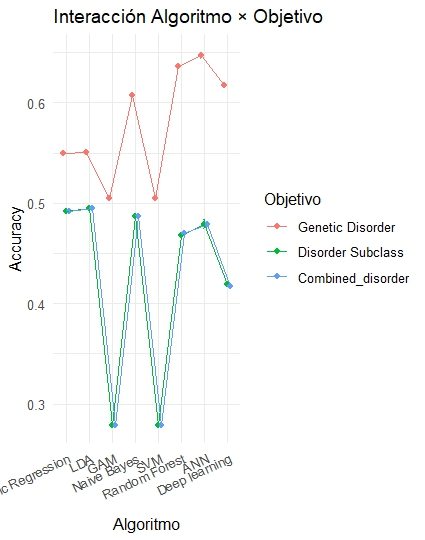
\includegraphics[width=0.5\linewidth]{Rplot01.jpeg}
    \caption{Interacción \textit{Algoritmo} $\times$ \textit{Objetivo} sobre \textit{Accuracy}.}
    \label{fig:interaccion_modelo_objetivo}
\end{figure}

\begin{table}[htbp]
\centering
\scriptsize
\caption{Resultados comparativos para \textit{Genetic Disorder}, \textit{Disorder Subclass} y \textit{Combined\_disorder}.}
\label{tab:resultados_completos}
\begin{tabular}{l l l r r r r r}
\toprule
Algoritmo & Objetivo & Arquitectura & Accuracy & Precision & Recall & F1\_score & Tiempo\_entrenamiento\_s \\
\midrule
Logistic Regression & Genetic Disorder & NA & 0.549 & 0.543 & 0.549 & 0.518 & 0.215 \\
Logistic Regression & Disorder Subclass & NA & 0.492 & 0.492 & 0.492 & 0.485 & 1.796 \\
Logistic Regression & Combined\_disorder & NA & 0.492 & 0.492 & 0.492 & 0.485 & 1.818 \\
LDA & Genetic Disorder & NA & 0.551 & 0.545 & 0.551 & 0.519 & 0.066 \\
LDA & Disorder Subclass & NA & 0.495 & 0.496 & 0.495 & 0.488 & 1.397 \\
LDA & Combined\_disorder & NA & 0.495 & 0.496 & 0.495 & 0.488 & 1.609 \\
GAM & Genetic Disorder & NA & 0.504 & 0.254 & 0.504 & 0.338 & 0.014 \\
GAM & Disorder Subclass & NA & 0.279 & 0.078 & 0.279 & 0.122 & 0.053 \\
GAM & Combined\_disorder & NA & 0.279 & 0.078 & 0.279 & 0.122 & 0.041 \\
Naive Bayes & Genetic Disorder & NA & 0.607 & 0.605 & 0.607 & 0.585 & 2.627 \\
Naive Bayes & Disorder Subclass & NA & 0.487 & 0.492 & 0.487 & 0.475 & 0.266 \\
Naive Bayes & Combined\_disorder & NA & 0.487 & 0.492 & 0.487 & 0.475 & 0.252 \\
SVM & Genetic Disorder & NA & 0.504 & 0.254 & 0.504 & 0.338 & 40.022 \\
SVM & Disorder Subclass & NA & 0.279 & 0.078 & 0.279 & 0.122 & 28.604 \\
SVM & Combined\_disorder & NA & 0.279 & 0.078 & 0.279 & 0.122 & 27.928 \\
Random Forest & Genetic Disorder & NA & 0.637 & 0.626 & 0.637 & 0.622 & 0.422 \\
Random Forest & Disorder Subclass & NA & 0.468 & 0.468 & 0.468 & 0.446 & 0.463 \\
Random Forest & Combined\_disorder & NA & 0.470 & 0.475 & 0.470 & 0.448 & 0.468 \\
ANN & Genetic Disorder & shallow & 0.643 & 0.636 & 0.643 & 0.637 & 17.261 \\
ANN & Genetic Disorder & medium & 0.643 & 0.639 & 0.643 & 0.638 & 8.061 \\
ANN & Genetic Disorder & deep & 0.652 & 0.660 & 0.652 & 0.654 & 8.216 \\
ANN & Genetic Disorder & dropout & 0.649 & 0.643 & 0.649 & 0.644 & 16.631 \\
ANN & Disorder Subclass & shallow & 0.482 & 0.478 & 0.482 & 0.474 & 9.614 \\
ANN & Disorder Subclass & medium & 0.474 & 0.477 & 0.474 & 0.462 & 8.036 \\
ANN & Disorder Subclass & deep & 0.471 & 0.483 & 0.471 & 0.466 & 7.776 \\
ANN & Disorder Subclass & dropout & 0.490 & 0.481 & 0.490 & 0.473 & 12.201 \\
ANN & Combined\_disorder & shallow & 0.483 & 0.483 & 0.483 & 0.474 & 8.968 \\
ANN & Combined\_disorder & medium & 0.479 & 0.481 & 0.479 & 0.474 & 7.400 \\
ANN & Combined\_disorder & deep & 0.470 & 0.467 & 0.470 & 0.460 & 7.243 \\
ANN & Combined\_disorder & dropout & 0.482 & 0.482 & 0.482 & 0.471 & 17.256 \\
Deep learning & Genetic Disorder & NA & 0.617 & 0.660 & 0.617 & 0.626 & 30.251 \\
Deep learning & Disorder Subclass & NA & 0.419 & 0.455 & 0.419 & 0.426 & 76.275 \\
Deep learning & Combined\_disorder & NA & 0.417 & 0.459 & 0.417 & 0.427 & 71.567 \\
\bottomrule
\end{tabular}
\end{table}

\section{Discusión}

\textbf{Contexto clínico y utilidad.} En detección temprana de enfermedades genéticas, la utilidad real de los modelos depende de su encaje en el flujo clínico, la estabilidad frente a datos heterogéneos y la facilidad de mantenimiento. Los enfoques estadísticos clásicos (p.ej., regresión logística, LDA, GAM, Naive Bayes) siguen siendo referencias sólidas en entornos sanitarios por su formulación bien establecida y despliegue ágil, además de su papel histórico como \emph{baseline} metodológico \cite{hosmer_2013,Hastie1986,10.1093/eurheartj/ehu207}. Por su parte, los métodos de inteligencia artificial (Random Forest, SVM, ANN y Deep Learning) permiten capturar estructuras no lineales y relaciones complejas típicas de la genética moderna, especialmente en escenarios multivariantes con fuertes interacciones \cite{Breiman2001,cortes1995,suykens1999,Libbrecht2015,LeCun_2015}. En la práctica clínica, ambos enfoques se utilizan de forma complementaria: modelos clásicos para decisiones rápidas y trazables, y modelos de IA para explotar patrones sutiles cuando la complejidad de los datos lo justifica \cite{Libbrecht2015,topol2019}.

\textbf{Robustez y escalabilidad ante alta dimensionalidad y datos incompletos.} En genética es habitual el régimen \emph{large $p$, small $n$}, con miles de predictores para un número limitado de pacientes. Los modelos clásicos requieren regularización, selección de variables y/o reducción de dimensión para mantener estabilidad y evitar sobreajuste \cite{10.1093/eurheartj/ehu207,CHEN2012}. LDA y regresión logística pueden degradarse cuando $p \gg n$ si no se aplican penalizaciones o controles adecuados; aun así, su sesgo estructural puede ser ventajoso cuando los datos son escasos y ruidosos \cite{dudoit2002}. En cambio, los métodos de \emph{machine learning} modernos ofrecen tolerancia intrínseca a la alta dimensionalidad: Random Forest realiza selección implícita de variables y atenúa la varianza mediante \emph{bagging} \cite{Breiman2001,CHEN2012,qi2012}; las SVM gestionan espacios de gran dimensión de forma controlada mediante el parámetro de margen y, si procede, núcleos no lineales \cite{cortes1995,suykens1999}. Las redes neuronales y el aprendizaje profundo aportan gran flexibilidad para modelar interacciones y no linealidades, pero requieren estrategias explícitas para prevenir el sobreajuste (p.ej., penalizaciones, \emph{dropout}) y suelen demandar más datos para estabilizarse \cite{LeCun_2015,Ching_2018}. En presencia de valores perdidos, todos los enfoques dependen de imputación u otras estrategias; los bosques aleatorios y ciertos \emph{pipelines} neuronales pueden integrar mejor estos mecanismos dentro del aprendizaje, mientras que los modelos lineales suelen exigir preprocesamientos más estrictos \cite{CHEN2012,Libbrecht2015}.

\textbf{Coste computacional e infraestructura.} Los métodos clásicos son ligeros en cómputo y memoria, lo que facilita su despliegue en sistemas hospitalarios convencionales y su actualización frecuente (reentrenos rápidos, integración sencilla en \emph{pipelines}) \cite{hosmer_2013,10.1093/eurheartj/ehu207}. Los algoritmos de IA, por el contrario, incrementan el coste tanto en entrenamiento como en inferencia: bosques grandes, SVM con núcleos y, especialmente, redes profundas requieren mayor capacidad de cómputo, optimización de hiperparámetros y, a menudo, aceleración por GPU \cite{Breiman2001,cortes1995,LeCun_2015}. En proyectos de cribado a gran escala (p.ej., programas poblacionales), las diferencias de latencia e infraestructura pueden ser determinantes para la adopción.

\textbf{Adaptabilidad a datos genéticos heterogéneos.} La integración de fuentes variadas (variantes genómicas, expresión, epigenética, analíticas clínicas, antecedentes) es un reto clave. Los enfoques clásicos requieren ingeniería de características y codificaciones explícitas (dummies, interacciones seleccionadas a priori), mientras que IA facilita esquemas de integración más flexibles: Random Forest maneja de forma natural variables mixtas; SVM se apoya en representaciones numéricas consistentes; y las redes profundas posibilitan arquitecturas multimodales que combinan módulos específicos (p.ej., secuencias, tabulares) y \emph{embeddings} para alta cardinalidad \cite{CHEN2012,Libbrecht2015,LeCun_2015,Ching_2018}. En la práctica, esta adaptabilidad de IA puede descubrir combinaciones novedosas de señales genéticas y clínicas, siempre que existan datos y validación suficiente \cite{Libbrecht2015,Ching_2018}.

\textbf{Aplicabilidad clínica, gobernanza y ciclo de vida.} Más allá del método, la aplicabilidad depende de validación externa, monitorización continua y gobernanza del modelo. En salud, los sistemas de IA se consideran de alto riesgo y están sujetos a requisitos de calidad de datos, trazabilidad y supervisión humana a lo largo de su ciclo de vida \cite{com2021laying,EC_AI_Act_2025}. Esto favorece marcos de despliegue escalables (control de versiones, auditorías, recalibración) donde los modelos clásicos, por su simplicidad, son más fáciles de auditar y mantener; los modelos complejos exigen procesos formales adicionales (documentación de datos, \emph{drift}, \emph{monitoring}) \cite{Libbrecht2015,topol2019}. En patologías genéticas, se han demostrado beneficios de IA en tareas específicas (p.ej., fenotipado facial o priorización de \emph{exomas}), lo que ilustra el potencial de enfoques avanzados cuando se integran en rutas clínicas bien definidas \cite{gurovich2019,Hsieh_2019}.

\textbf{Ventajas, limitaciones y enfoque híbrido.} No existe un único ``ganador'' universal. Los métodos clásicos aportan rapidez, estabilidad y facilidad de gobierno; IA ofrece capacidad de modelado para patrones complejos y datos heterogéneos, a costa de mayor complejidad operativa. Un flujo híbrido resulta pragmático: utilizar modelos clásicos como primera capa de cribado y priorización, y reservar modelos avanzados (RF, SVM, DL) para casos ambiguos o cuando se disponga de información ómica rica \cite{Breiman2001,cortes1995,Libbrecht2015,LeCun_2015}. La elección óptima dependerá de: (i) disponibilidad y calidad de datos, (ii) requisitos de latencia e infraestructura, (iii) exigencias regulatorias y de mantenimiento, y (iv) criticidad clínica del uso previsto \cite{10.1093/eurheartj/ehu207,EC_AI_Act_2025}. 

\textbf{Implicaciones para este trabajo.} Dado que el estudio no se centra en precisión ni en interpretabilidad, la comparación crítica se ha orientado a aplicabilidad clínica, robustez, coste computacional y adaptabilidad a datos genéticos. En este marco, los resultados y la experiencia de entrenamiento apuntan a que los métodos clásicos son idóneos como referencia y despliegue inicial, mientras que los modelos de IA aportan valor diferencial cuando existen suficientes datos y un ecosistema de validación y operación capaz de sostener su complejidad \cite{Libbrecht2015,Ching_2018,topol2019}.

\section{Conclusiones y Trabajo Futuro}

\noindent \textbf{Resumen de hallazgos principales.} En este estudio se han comparado métodos estadísticos clásicos (regresión logística, Análisis Discriminante Lineal, GAM, Naive Bayes) con técnicas modernas de inteligencia artificial (Random Forest, SVM, redes neuronales y aprendizaje profundo) para la detección temprana de enfermedades genéticas. Cualitativamente, ambos enfoques muestran fortalezas diferenciadas pero complementarias. Los modelos estadísticos tradicionales destacan por su sencillez e interpretabilidad, lo que les confiere una sólida aceptación en entornos clínicos \cite{10.1093/eurheartj/ehu207}. Su formulación bien establecida facilita la validación y el despliegue, actuando a menudo como referentes o líneas base en problemas biomédicos. Por otro lado, los métodos de \textit{machine learning} e inteligencia artificial ofrecen mayor capacidad para capturar patrones no lineales y estructuras complejas presentes en datos genéticos \cite{Breiman2001,Libbrecht2015,LeCun_2015}. Técnicas como Random Forest o las redes neuronales profundas pueden modelar interacciones sutiles entre múltiples variables (genéticas, clínicas, ambientales) que podrían pasar desapercibidas bajo supuestos lineales. En consecuencia, no se encontró un método “universalmente superior” en todos los aspectos; cada familia de modelos mostró un desempeño destacado bajo ciertas condiciones de los datos y objetivos. Esto refuerza la noción de que la elección óptima depende del contexto: los modelos estadísticos clásicos proveen rapidez de cómputo y transparencia, útiles para decisiones inmediatas y trazables, mientras que los modelos de IA aportan potencia predictiva cuando la complejidad de los datos lo justifica \cite{Libbrecht2015,10.1093/eurheartj/ehu207}. En la práctica clínica, estos enfoques pueden utilizarse de forma complementaria: técnicas simples para un primer cribado interpretable y modelos avanzados para explotar patrones más complejos que mejoren la detección \cite{Libbrecht2015,topol2019}.

\noindent \textbf{Recomendaciones prácticas.} Derivado de los hallazgos, recomendamos una adopción progresiva y equilibrada de ambas aproximaciones en entornos clínicos y de desarrollo. Dado que en el diagnóstico genético la interpretabilidad y confiabilidad son esenciales, resulta prudente comenzar evaluando modelos estadísticos sencillos (p.~ej., regresión logística) como herramientas de cribado o apoyo inicial, ya que permiten explicar fácilmente las predicciones a los especialistas \cite{10.1093/eurheartj/ehu207,rudin_2019}. Si el problema en cuestión involucra relaciones no lineales complejas o gran dimensionalidad de los datos, entonces la incorporación de modelos de IA más sofisticados está justificada, siempre y cuando se cuente con datos suficientes para entrenarlos adecuadamente \cite{Ching_2018,Libbrecht2015}. En estos casos, es fundamental aplicar validaciones rigurosas (validación cruzada, conjuntos externos) para garantizar la robustez del modelo y evitar sobreajuste, así como emplear estrategias de \textit{interpretabilidad} que permitan extraer conocimiento del modelo automático (por ejemplo, estimar la importancia de variables en un Random Forest o usar técnicas de explicación como SHAP/LIME en redes neuronales) \cite{rudin_2019}. De este modo, incluso los algoritmos de tipo ``caja negra'' pueden brindar información trazable que facilite su aceptación por parte del personal médico. Igualmente, se debe considerar la viabilidad computacional y operacional: los modelos basados en deep learning implican mayores requerimientos de cómputo y tiempo de entrenamiento, por lo que su implementación requerirá infraestructura adecuada (GPUs, servidores) y un plan de mantenimiento que supervise el rendimiento del modelo a lo largo del tiempo. Por último, cabe destacar que cualquier herramienta desarrollada debe alinearse con las regulaciones y guías éticas emergentes para IA en salud (p.~ej., exigencias de transparencia y gestión de riesgo definidas en el futuro Reglamento Europeo de IA), garantizando así que su uso clínico sea seguro, efectivo y conforme a la normativa vigente.

\noindent \textbf{Limitaciones del estudio.} Si bien el estudio aporta evidencias sobre las ventajas y desafíos de cada enfoque, es importante reconocer sus limitaciones. En primer lugar, el conjunto de datos empleado (proveniente de una competición pública) podría no representar completamente la casuística real de las enfermedades genéticas en la población general. El tamaño muestral relativamente reducido, junto con la presencia de clases minoritarias, limita la potencia estadística y podría sesgar las conclusiones hacia las características particulares de estos datos. Muchos trastornos genéticos –especialmente enfermedades raras– cuentan con muy pocos casos documentados, lo cual dificulta entrenar modelos fiables y generalizables \cite{Libbrecht2015,Ching_2018}. En nuestro caso, la escasez y posible falta de diversidad en los datos podrían haber favorecido a métodos con mayor sesgo inductivo (modelos lineales) frente a otros más flexibles, o viceversa, según la estructura del ruido presente. En segundo lugar, no se dispuso de un conjunto de validación verdaderamente externo para evaluar la generalización fuera de muestra. Esto implica que los resultados obtenidos (p.~ej., en métricas de clasificación) pueden estar optimizados para este \textit{dataset} específico, y su rendimiento podría degradar en datos de otros orígenes. Una validación externa independiente habría fortalecido la evidencias sobre qué método resulta más consistente, siguiendo las buenas prácticas de desarrollo de modelos predictivos clínicos \cite{10.1093/eurheartj/ehu207}. Asimismo, el enfoque comparativo se centró principalmente en métricas de exactitud predictiva, sin incorporar análisis exhaustivos de calibración, utilidad clínica o coste-efectividad de cada modelo. Aspectos prácticos como el tiempo de inferencia, la facilidad de integración en flujos clínicos o la aceptación por parte del usuario final no fueron cuantificados en este trabajo, pero sin duda influyen en el éxito de una herramienta diagnóstica y merecen consideración. Por último, cabe mencionar que la optimización de hiperparámetros y arquitecturas fue limitada en algunos casos (especialmente para las redes neuronales profundas, donde se probaron configuraciones estándar). Es posible que con una búsqueda más amplia o técnicas de ajuste más avanzadas (p.~ej., \textit{Bayesian optimization} para hiperparámetros, o \textit{AutoML}) se pudiera mejorar el rendimiento de ciertos algoritmos, por lo que las diferencias observadas entre métodos no deben interpretarse como absolutas. Del mismo modo, no exploramos a fondo métodos de ensamble o combinaciones híbridas de modelos, que potencialmente podrían aprovechar lo mejor de cada enfoque. Estas limitaciones abren oportunidades para refinar y extender el trabajo en el futuro.

\noindent \textbf{Líneas futuras de trabajo.} A partir de las limitaciones y hallazgos mencionados, se proponen varias direcciones para la continuación y mejora de este trabajo. En primer lugar, resulta imprescindible ampliar el volumen y la diversidad de los datos disponibles. Es necesario construir o acceder a conjuntos de datos más grandes, heterogéneos y representativos de la población (incluyendo distintas etnias, edades y variabilidad genómica) a fin de entrenar modelos más robustos y reducir el riesgo de sesgos en las predicciones \cite{Libbrecht2015,Ching_2018}. Iniciativas de colaboración multi-centro y bancos de datos compartidos podrían facilitar este objetivo, al igual que técnicas de data augmentation (por ejemplo, generar variaciones sintéticas de muestras existentes) que ya han mostrado mejorar notablemente el rendimiento diagnóstico cuando se incrementa la información de entrenamiento \cite{topol2019}. En segundo lugar, se propone avanzar hacia la integración de datos multimodales en los modelos. La detección temprana de enfermedades genéticas podría beneficiarse de combinar datos genómicos con otras fuentes complementarias, como historiales clínicos, imágenes médicas o fenotipos físicos del paciente. Esta integración ofrecería una visión más holística del caso, permitiendo al algoritmo aprovechar tanto la información molecular como las manifestaciones observables de la enfermedad \cite{Ching_2018}. Por ejemplo, recientes estudios han demostrado que el análisis automatizado de rasgos faciales mediante deep learning puede contribuir al diagnóstico de síndromes genéticos con fenotipos característicos, cuando se usa junto con la secuenciación genética \cite{gurovich2019}. Implementar modelos que fusionen estas modalidades (datos clínicos + genómicos + imágenes) es un paso natural para aumentar la precisión diagnóstica, aunque conlleva retos importantes en cuanto a arquitectura de red, normalización de datos heterogéneos y requerimientos computacionales. En tercer lugar, es prioritario desarrollar métodos que mejoren la interpretabilidad de los modelos de inteligencia artificial aplicados a genética. La falta de explicaciones claras de las predicciones puede obstaculizar la confianza y adopción de modelos complejos en medicina \cite{rudin_2019}. Por ende, futuras investigaciones deberían centrarse en técnicas explicativas específicas para este dominio, tales como identificar qué variantes genéticas, regiones del genoma o variables clínicas están dominando la decisión de un modelo dado \cite{Ching_2018}. Esto podría lograrse mediante algoritmos poshoc de interpretabilidad (p.~ej., visualización de gradients en redes profundas, descomposición de aportes en modelos de árbol) o, alternativamente, diseñando modelos intrínsecamente interpretables que incorporen conocimiento experto (por ejemplo, reglas clínicas o vías biológicas conocidas) junto con el aprendizaje automático \cite{Alsentzer2025}. El desarrollo de sistemas híbridos neuro-simbólicos o enfoques de \textit{autoML} con restricciones de interpretabilidad son vías prometedoras a explorar. Finalmente, se recomienda acercar estas soluciones al entorno real mediante evaluaciones clínicas prospectivas. Un paso futuro crucial consiste en integrar los modelos propuestos en estudios clínicos piloto o programas de tamizaje genético, donde se pueda medir su desempeño e impacto en tiempo real. Esto implicaría no sólo verificar la precisión diagnóstica en la práctica, sino también evaluar cómo la herramienta influye en la toma de decisiones del médico, en los tiempos de diagnóstico y en la experiencia del paciente. Adicionalmente, sería valioso analizar la relación coste-beneficio de implementar estas tecnologías en el sistema sanitario (por ejemplo, si ayudan a evitar pruebas invasivas o diagnósticos erróneos, justificando su coste computacional). A medida que se avance en este camino, deberá asegurarse la actualización continua de los modelos con nuevos datos (aprendizaje continuo) para mantener su vigencia, y el cumplimiento estricto de las normativas de privacidad de datos y de inteligencia artificial ética. En suma, las líneas futuras se orientan a (i) enriquecer los datos disponibles, (ii) aprovechar la información multimodal, (iii) lograr modelos más interpretables, y (iv) validar exhaustivamente su utilidad en la práctica clínica real, con el objetivo último de mejorar la detección precoz de enfermedades genéticas de manera segura, eficaz y equitativa.


\bibliographystyle{apacite}
\bibliography{bibliografia}

\appendix
\chapter{Apendices}

El código desarrollado para este trabajo, junto con scripts de preprocesamiento y experimentación, se encuentra disponible en el siguiente repositorio de GitHub: \\
\url{https://github.com/fobos01/TFM}
\end{document}





















